\section{Operating VICON}
\label{sec:OperatingVICON}
\subsection{The Hardware}
\label{sec:viconsetup}
From within the Cranfield flight arena, this is the current hardware setup for the VICON positioning system. Image \ref{fig:hardwareReference} is your reference for the name I uses throughout this guide. 
\begin{figure}[H]
        \centering
        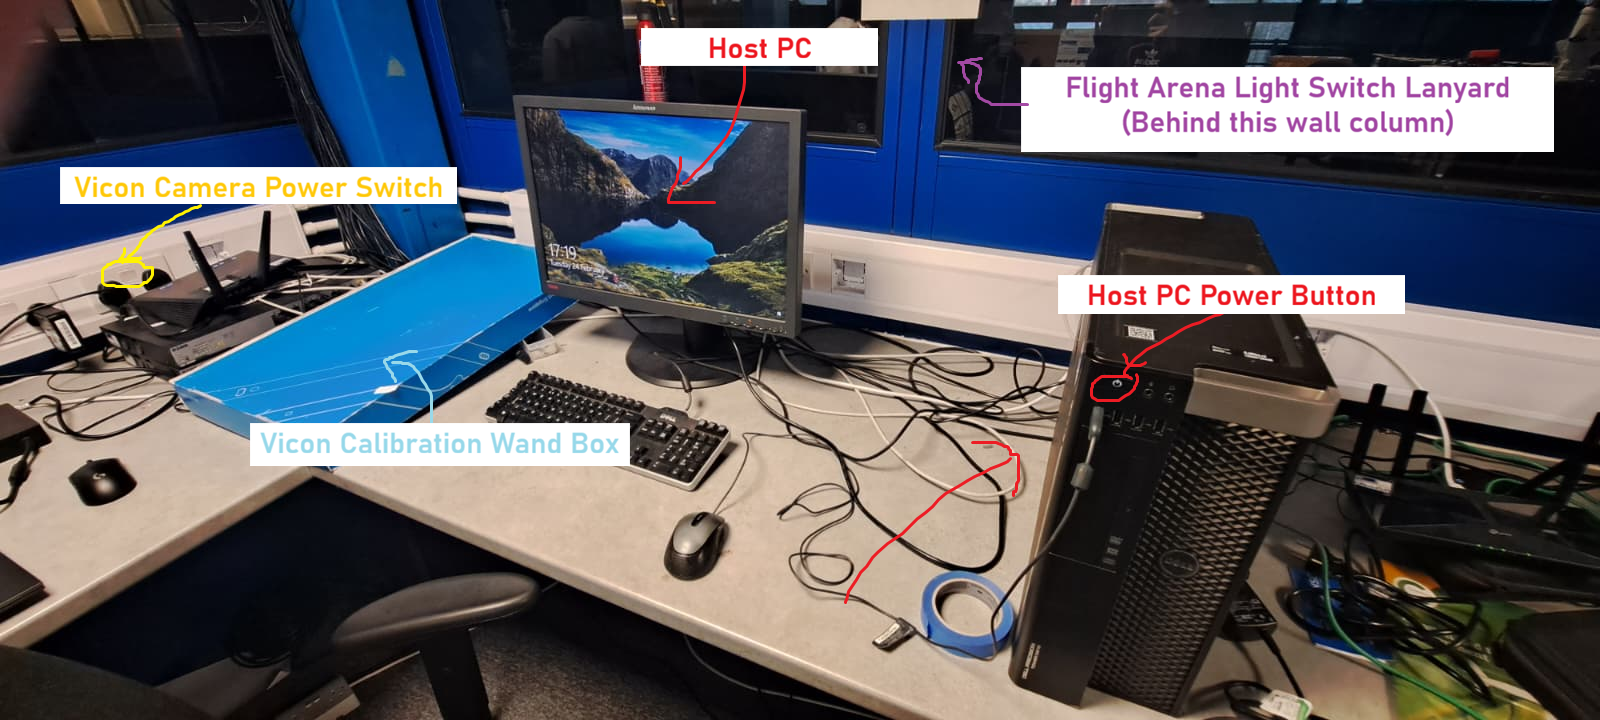
\includegraphics[width=1\linewidth]{Images/Overall Hardware.png}
        \caption{Overall VICON Hardware Architecture}
        \label{fig:hardwareReference}
\end{figure}
\subsection{Turn on Vicon cameras and Host PC}
To use the Vicon, firstly, on the corner of the wall, switch on both of the VICON Camera Power Switch. \textbf{Wait 20 minutes for the Camera to warmup.} Meanwhile, turn on the VICON Host PC by pressing the Host PC Power Button. Log into the computer, when asked for the password, it is \textbf{"Cranfield01"}. Once logged in, launch the "Vicon Tracker 3.10.0 x64" app. 
\begin{figure}[H]
    \centering
    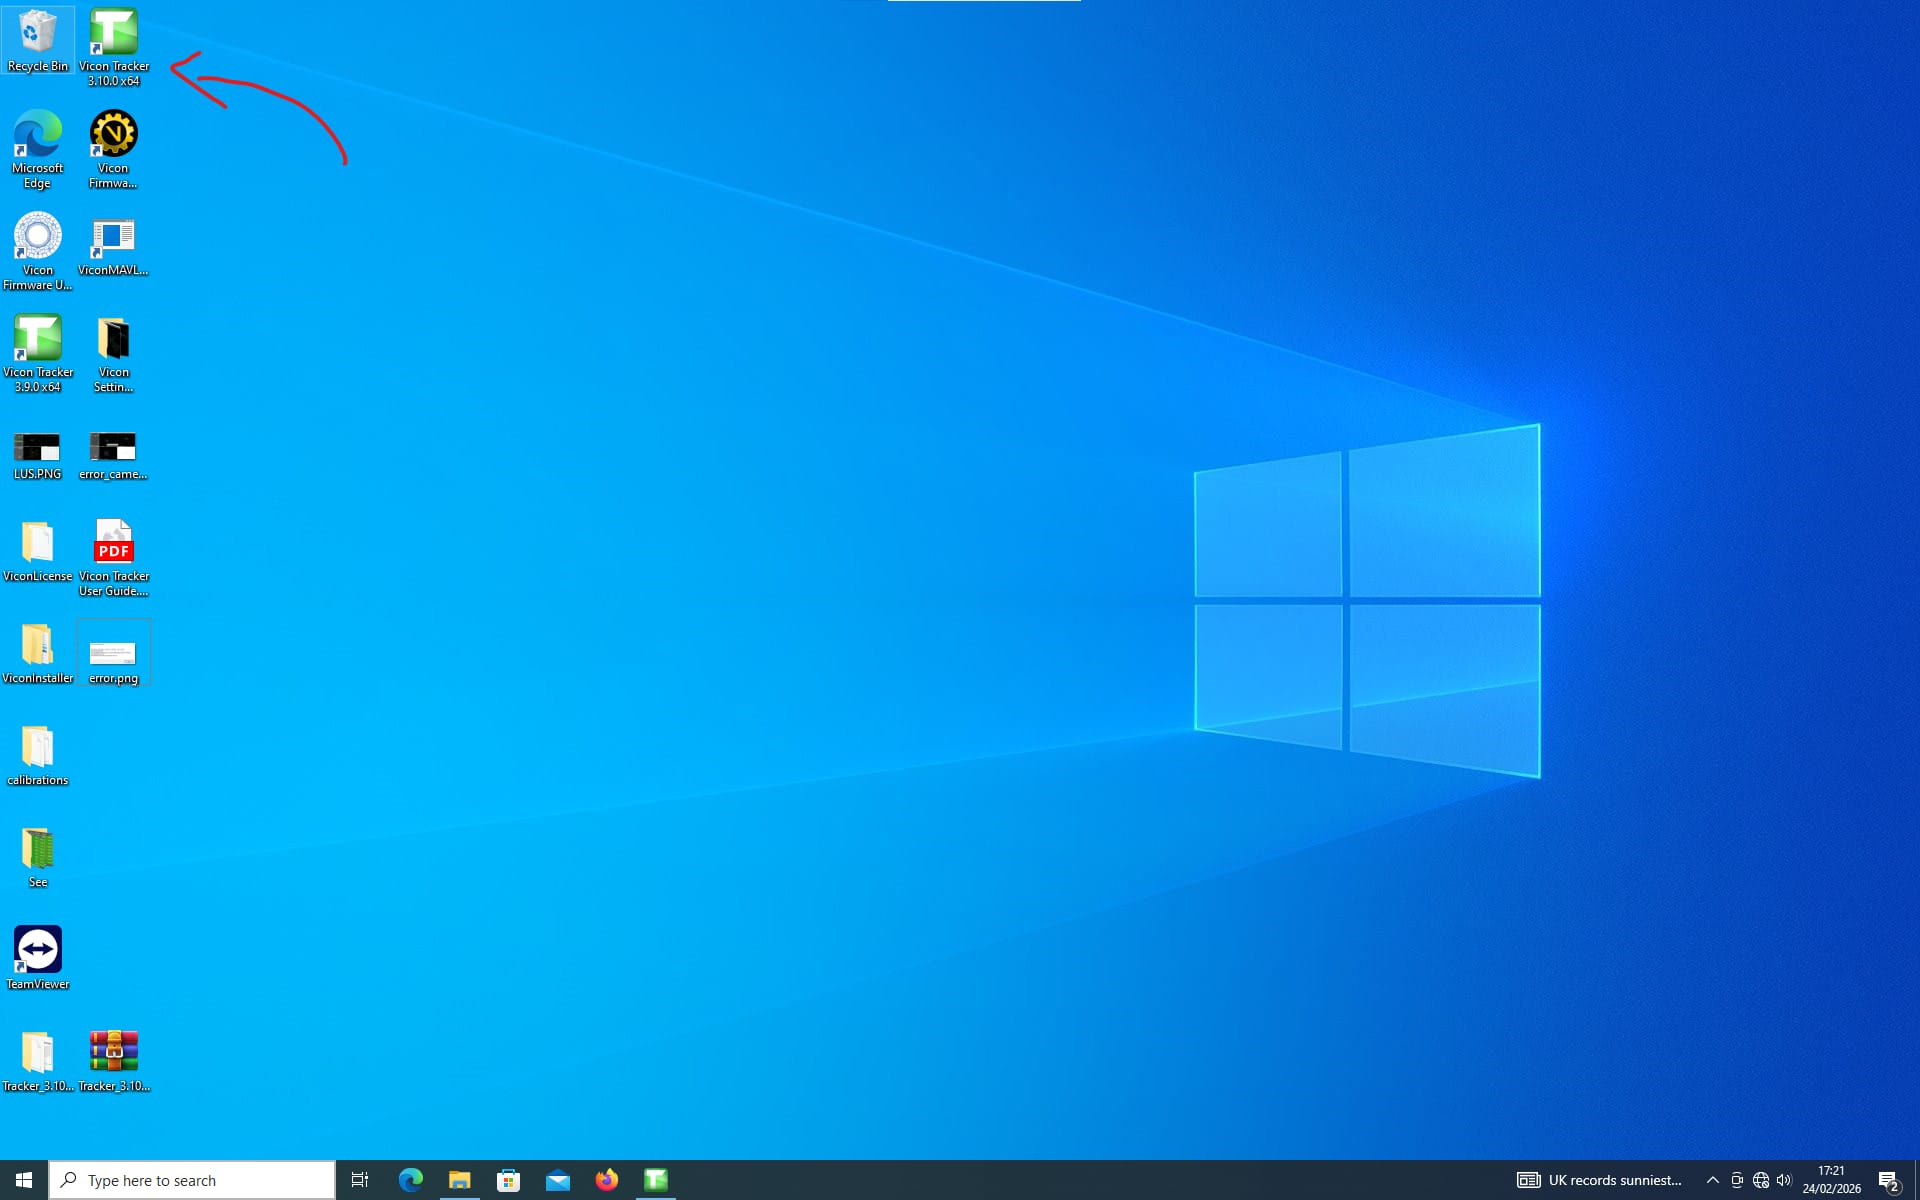
\includegraphics[width=0.7\linewidth]{Images/WhatsApp Image 2026-02-24 at 19.06.15.jpeg}
    \caption{Image of desktop and the app's corresponding location.}
\end{figure}
App will launch, focus on the left side of the app as seen in figure \ref{fig:viconwhere}, and navigate to the \textit{SYSTEM} tab. After 20 minutes of warmup, verify that all cameras under \textit{Vicon Camera} are good and without yellow or red crosses. 
\begin{figure}[H]
    \centering
    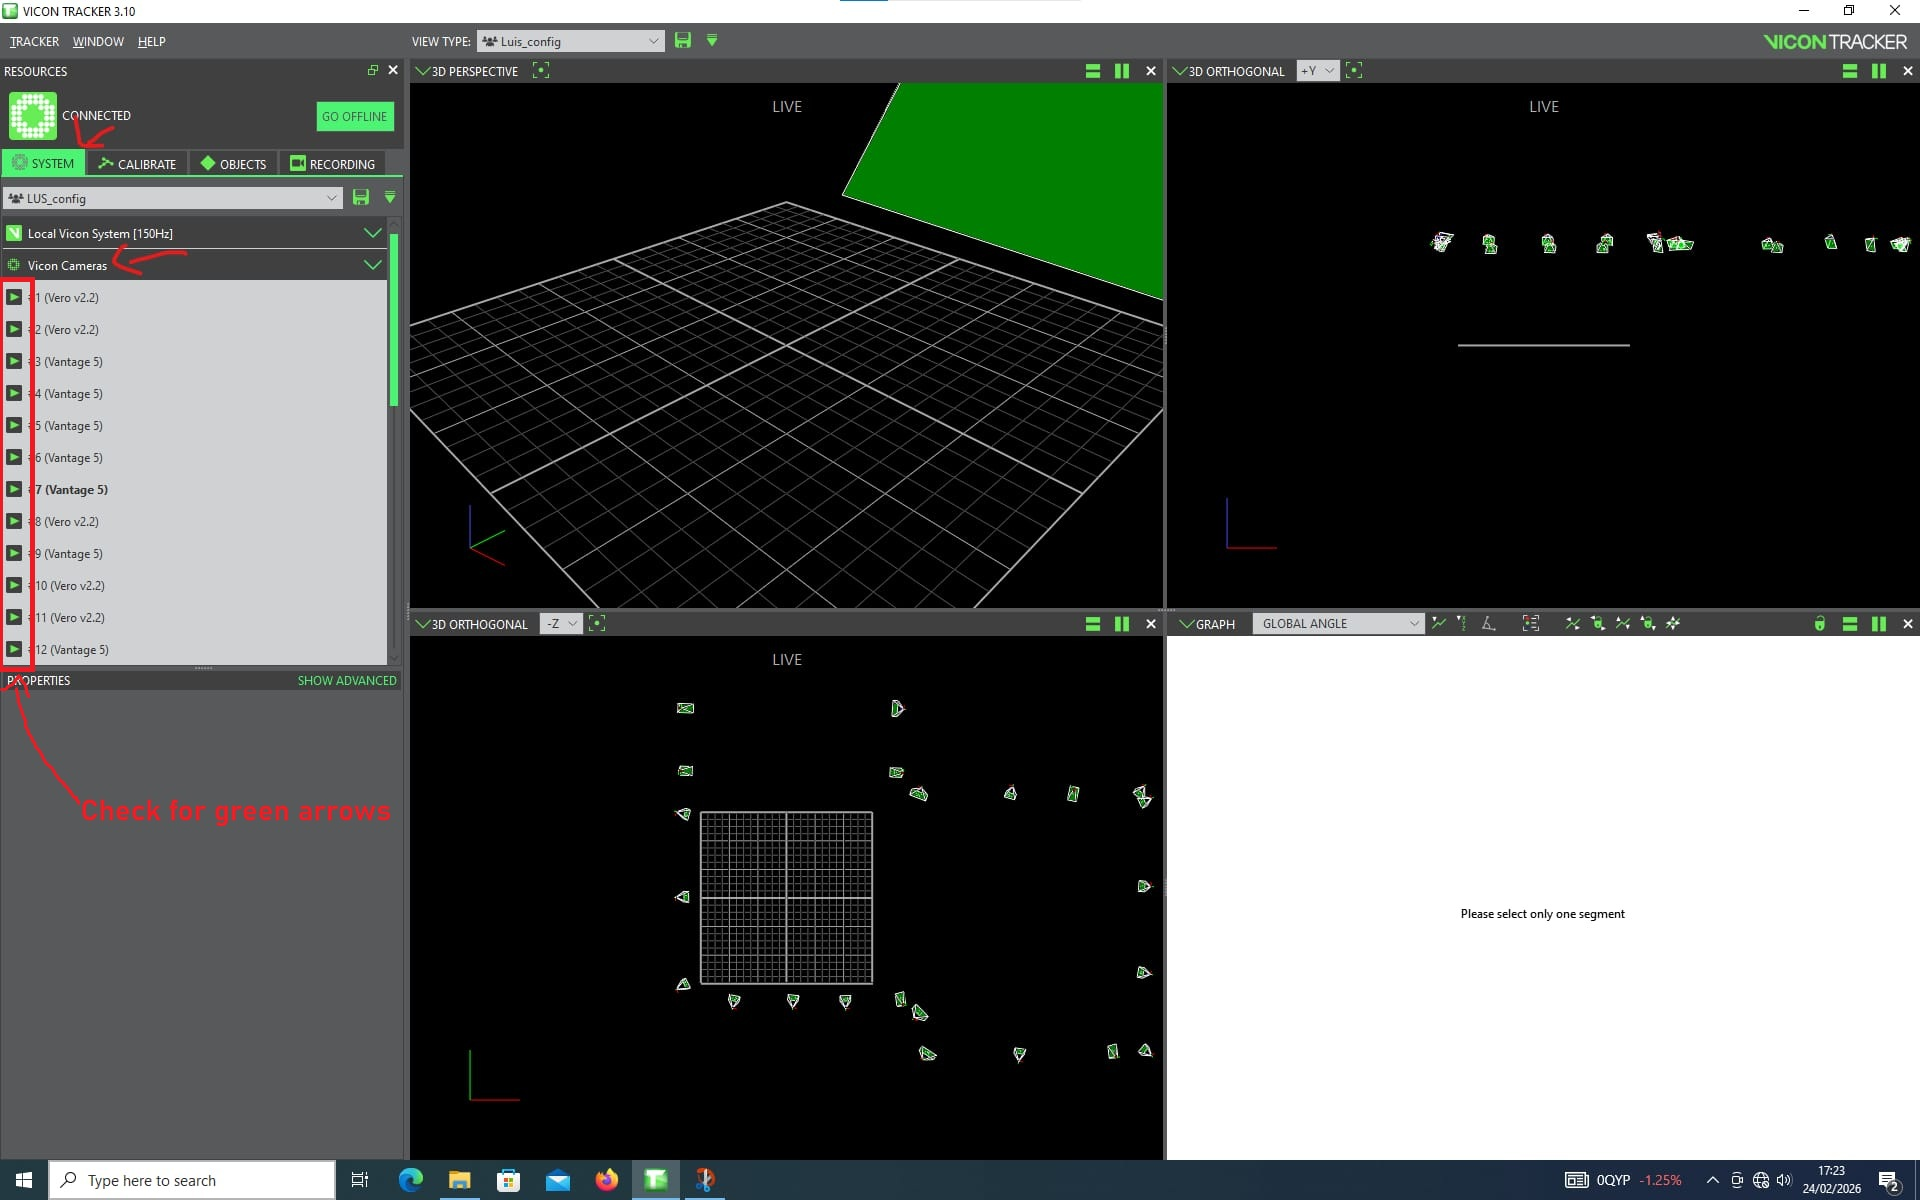
\includegraphics[width=0.95\linewidth]{Images/WhatsApp Image 2026-02-24 at 19.06.16 (3).jpeg}
    \caption{Image of "SYSTEM TAB" and verification of camera after warmup.}
    \label{fig:viconwhere}
\end{figure}
If cameras are not ready, click on \textit{Local Vicon System [150Hz]} $\to$ \textit{PROPERTIES} $\to$ \textit{REBOOT ALL}, as seen in figure \ref{fig:5} below.

\begin{figure}[H]
    \centering
    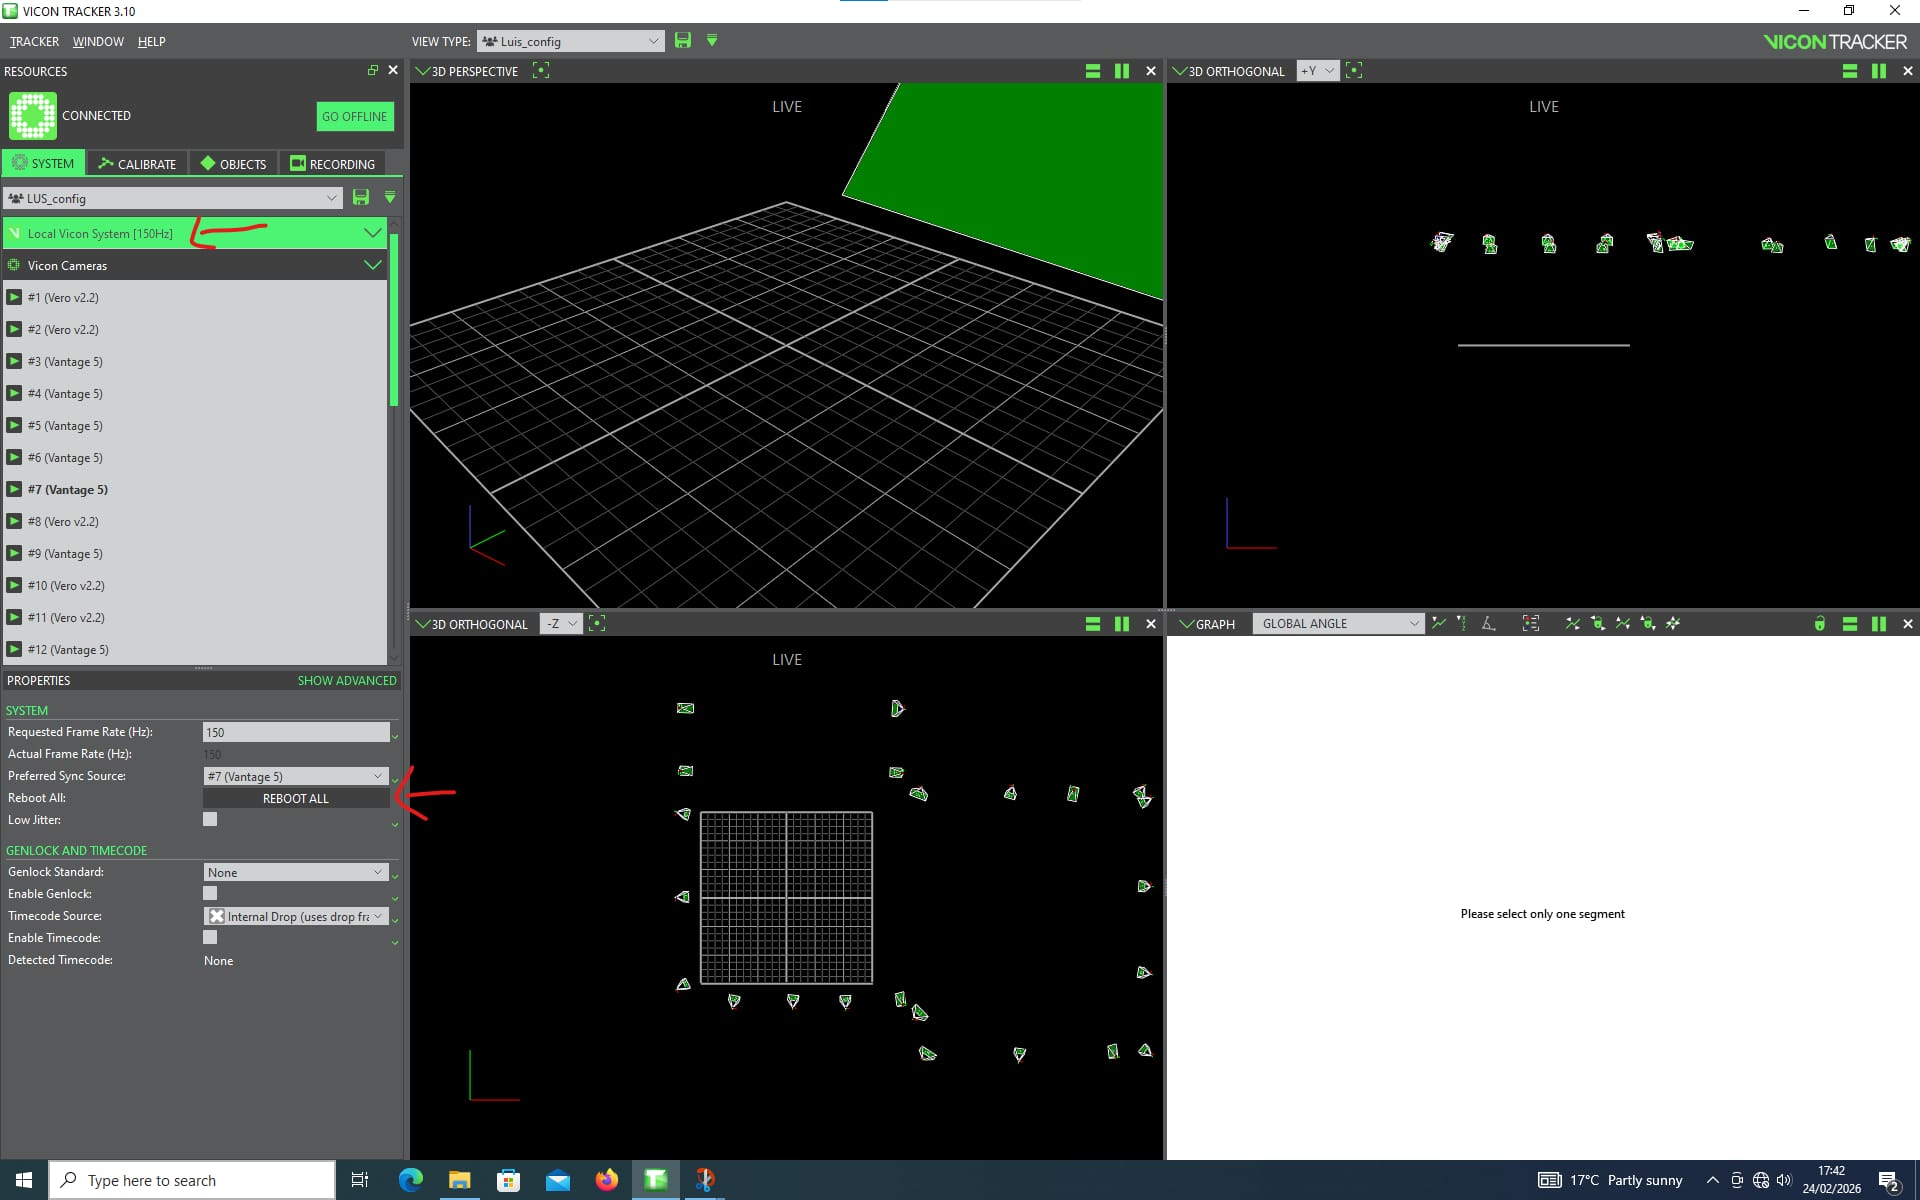
\includegraphics[width=0.9\linewidth]{Images/WhatsApp Image 2026-02-24 at 19.06.17.jpeg}
    \caption{Image of \textit{SYSTEM} tab.}
    \label{fig:5}
\end{figure}

\subsection{Create a Camera Mask}
Navigate to the \textit{CALIBRATE} tab next to \textit{SYSTEM} tab. Create a camera mask by pressing \textit{START} under \textit{CREATE CAMERA MASK} as seen in figure \ref{fig:6}. This masks takes a snapshot of the environment and filters out any IR reflection it sees from the environment. \footnote{If your testing have any obstacles, put them in physically before creating a camera mask. Also, make sure you turn on the flight arena lights!}\\ 
\vspace{0.2cm}

\begin{figure}[H]
    \centering
    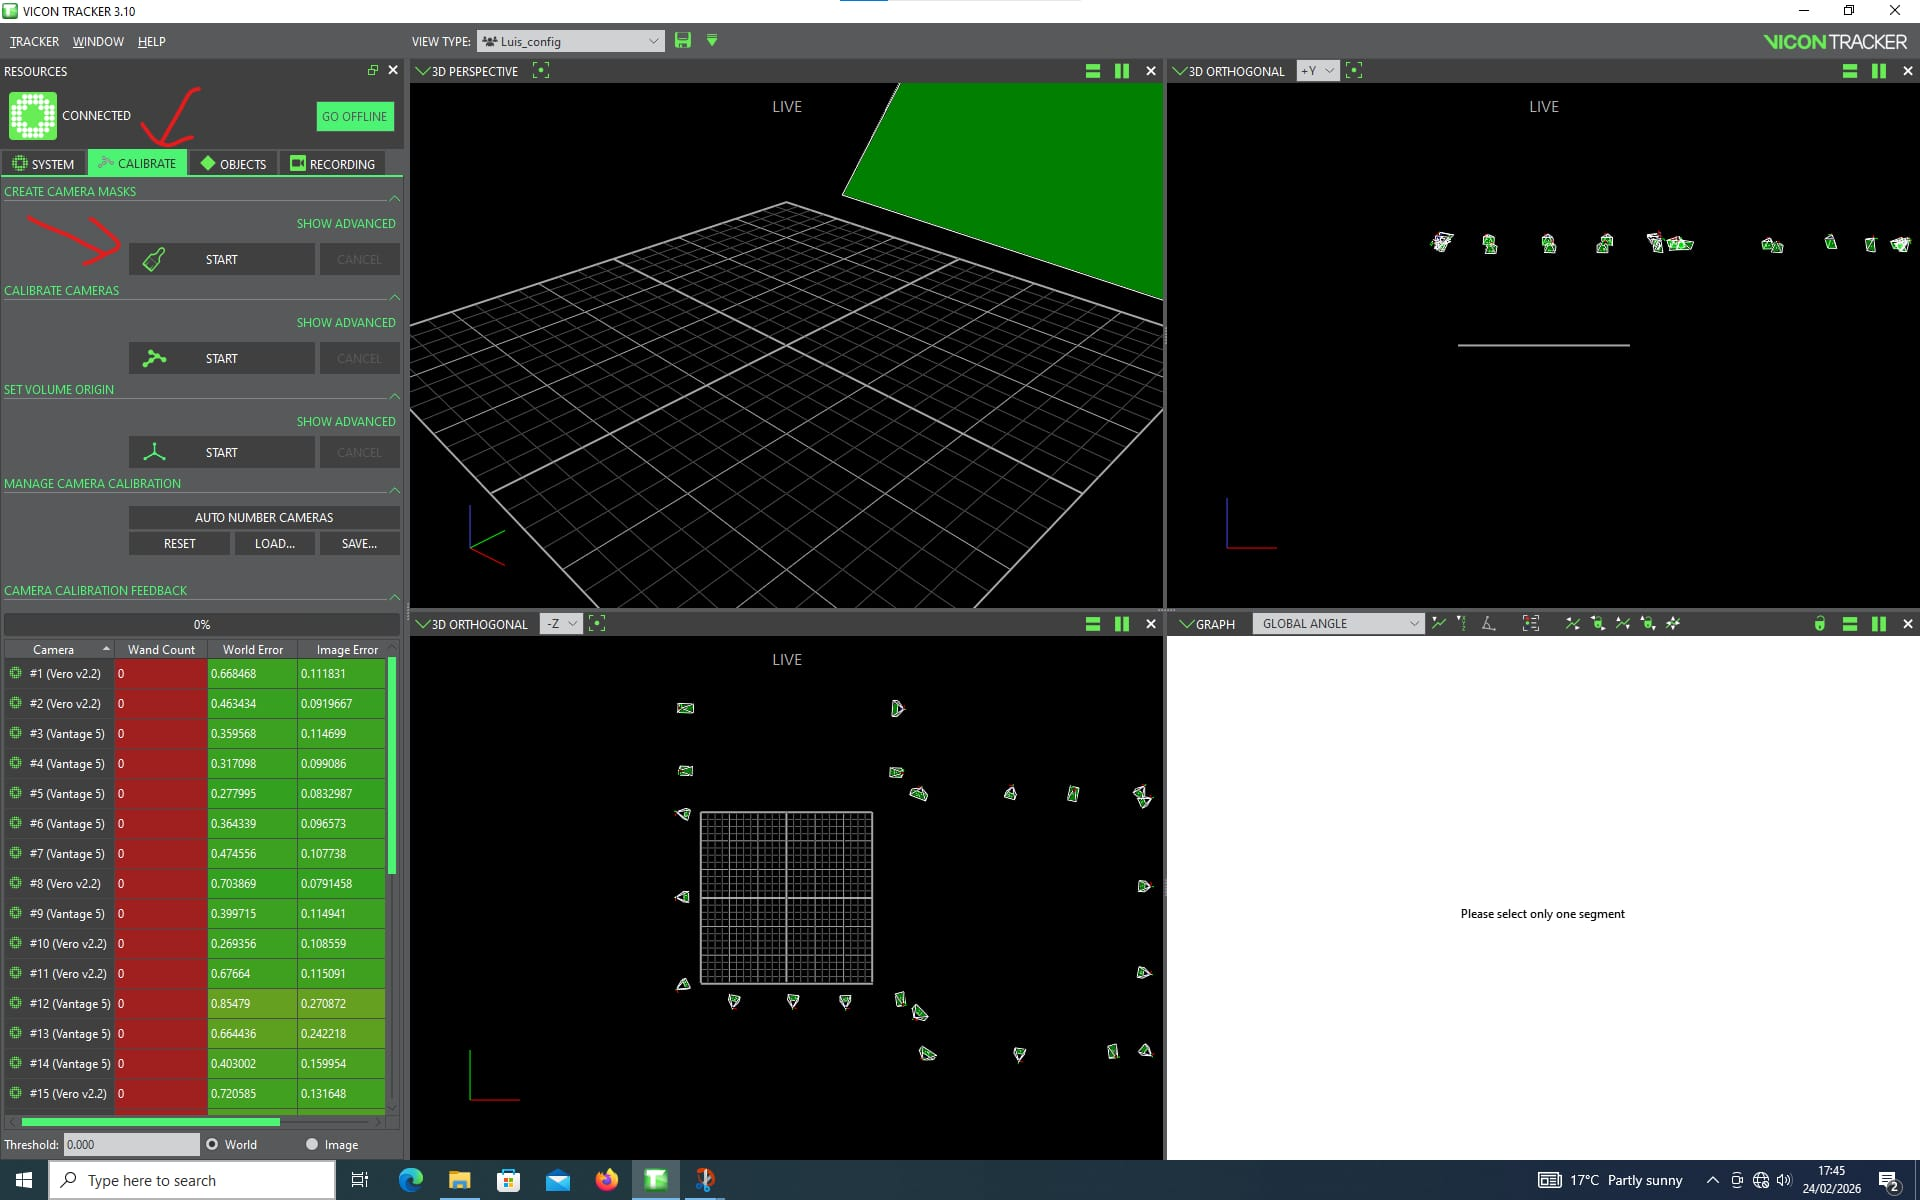
\includegraphics[width=0.8\linewidth]{Images/WhatsApp Image 2026-02-24 at 19.06.17 (1).jpeg}
    \caption{Image of \textit{CALIBRATE} tab and Camera Masks button.}
    \label{fig:6}
\end{figure}

The blue pixels highlighted on each individual camera views are the IR reflection the camera spotted from within the environment. Once the blue dots stops changing much, press \textit{STOP}. (If any cameras have complete blue screens, that means something is wrong and a camera reboot/power flushing the cameras is needed.) 

\begin{figure}[H]
    \centering
    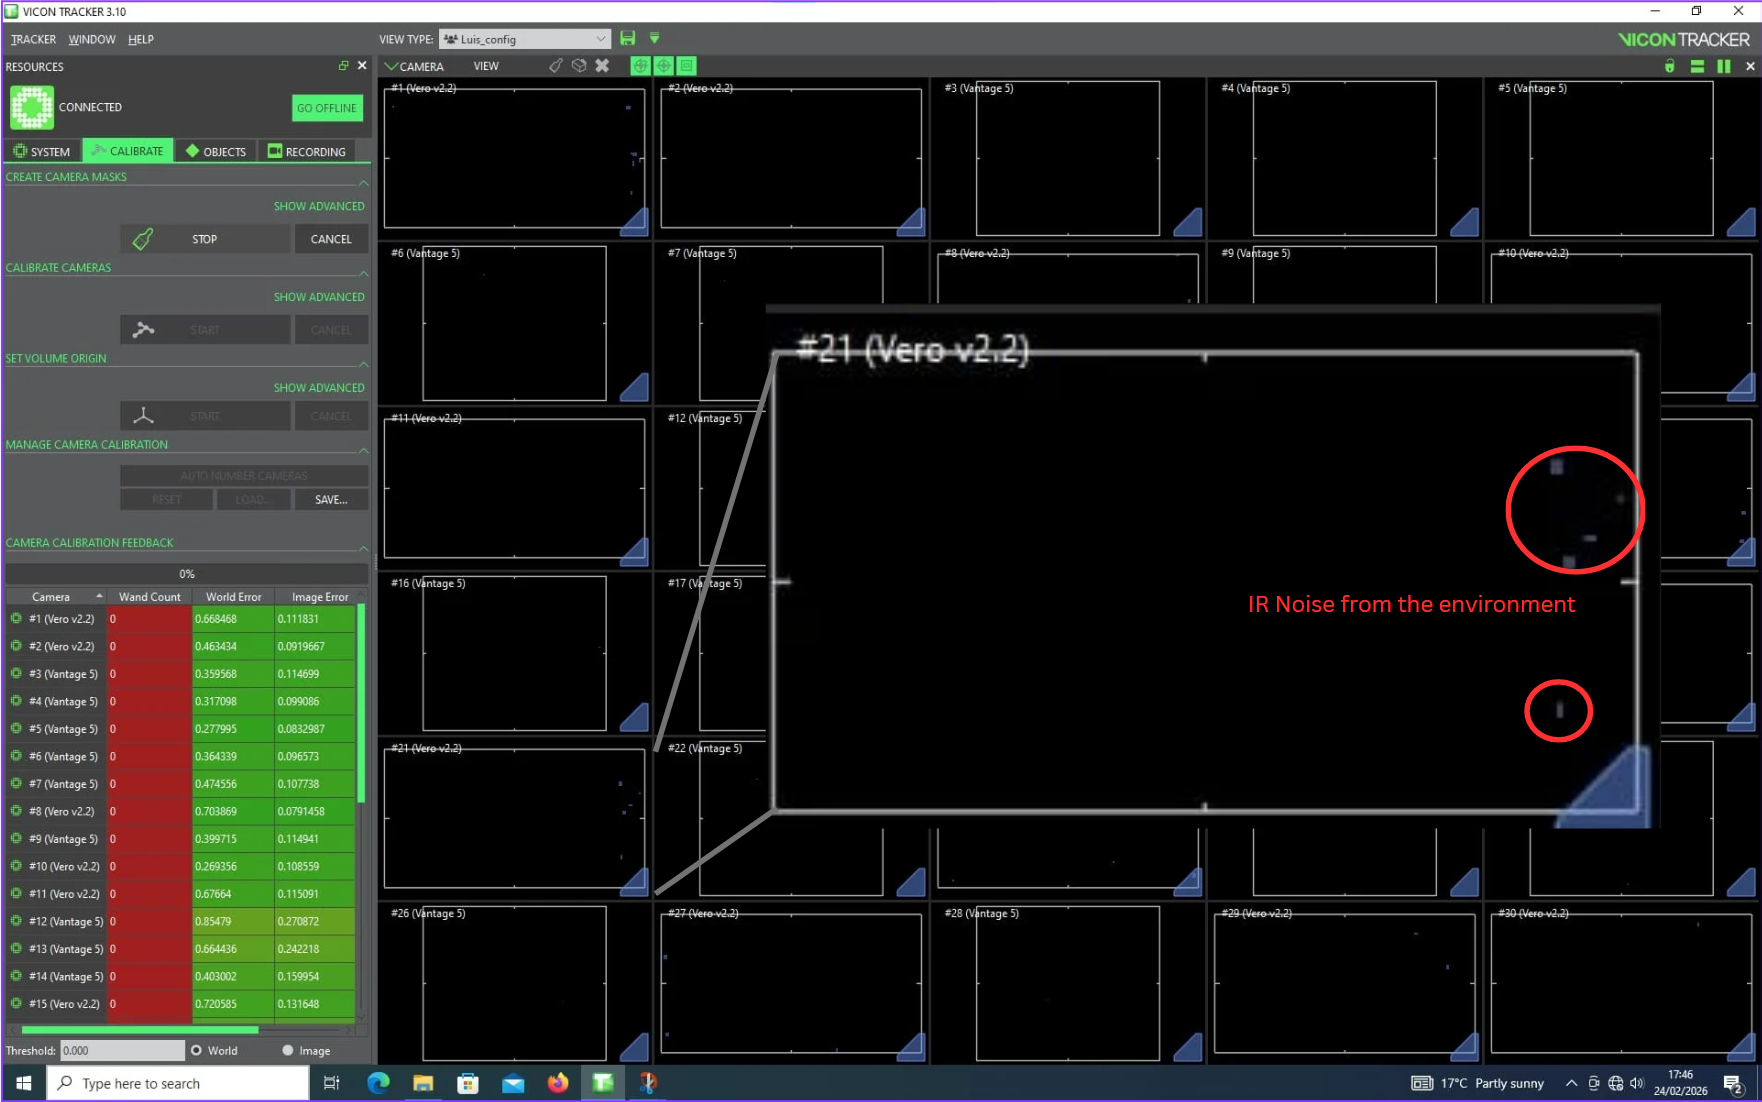
\includegraphics[width=0.8\linewidth]{Images/NoiseGeneration.png}
    \caption{Image of Camera Mask being created and the corresponding \textit{STOP} button.}
\end{figure}

\subsection{How to turn on the lights of Flight Arena}
\label{sec:lights}
To turn on the lights, physically enter your biological body into the flight arena, walk towards the wall that faces the Host PC. Find the light switch lanyard (Yes a lanyard, not a button), aim it towards the lights on top, click the yellow button. 

\begin{figure}[H]
    \centering
    \begin{subfigure}[b]{0.32\linewidth}
        \centering
        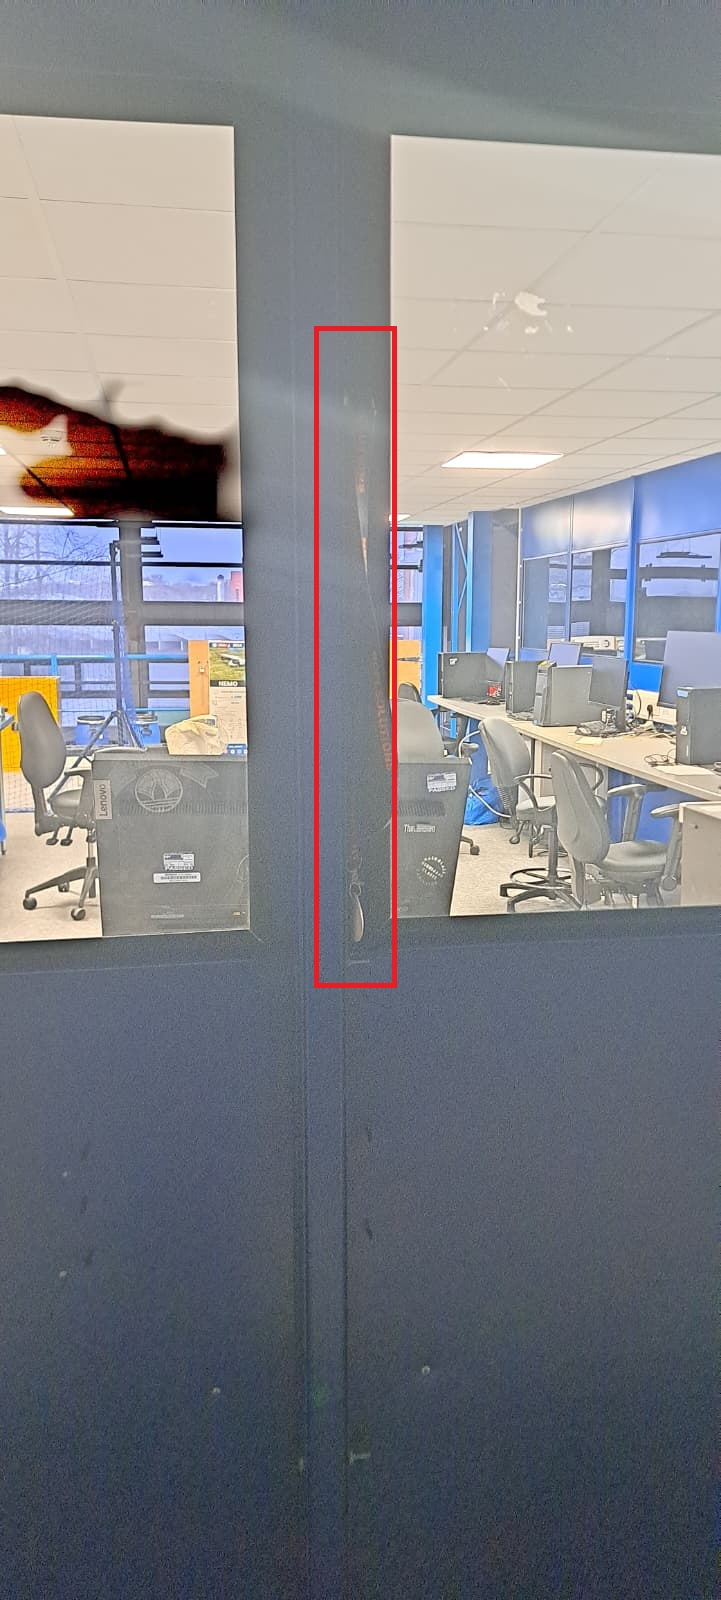
\includegraphics[width=\linewidth]{Images/WhatsApp Image 2026-02-24 at 19.05.02 (1).jpeg}
        \caption{Location of Flight Arena Light Switch Lanyard.}
    \end{subfigure}
    \hfill
    \begin{subfigure}[b]{0.32\linewidth}
        \centering
        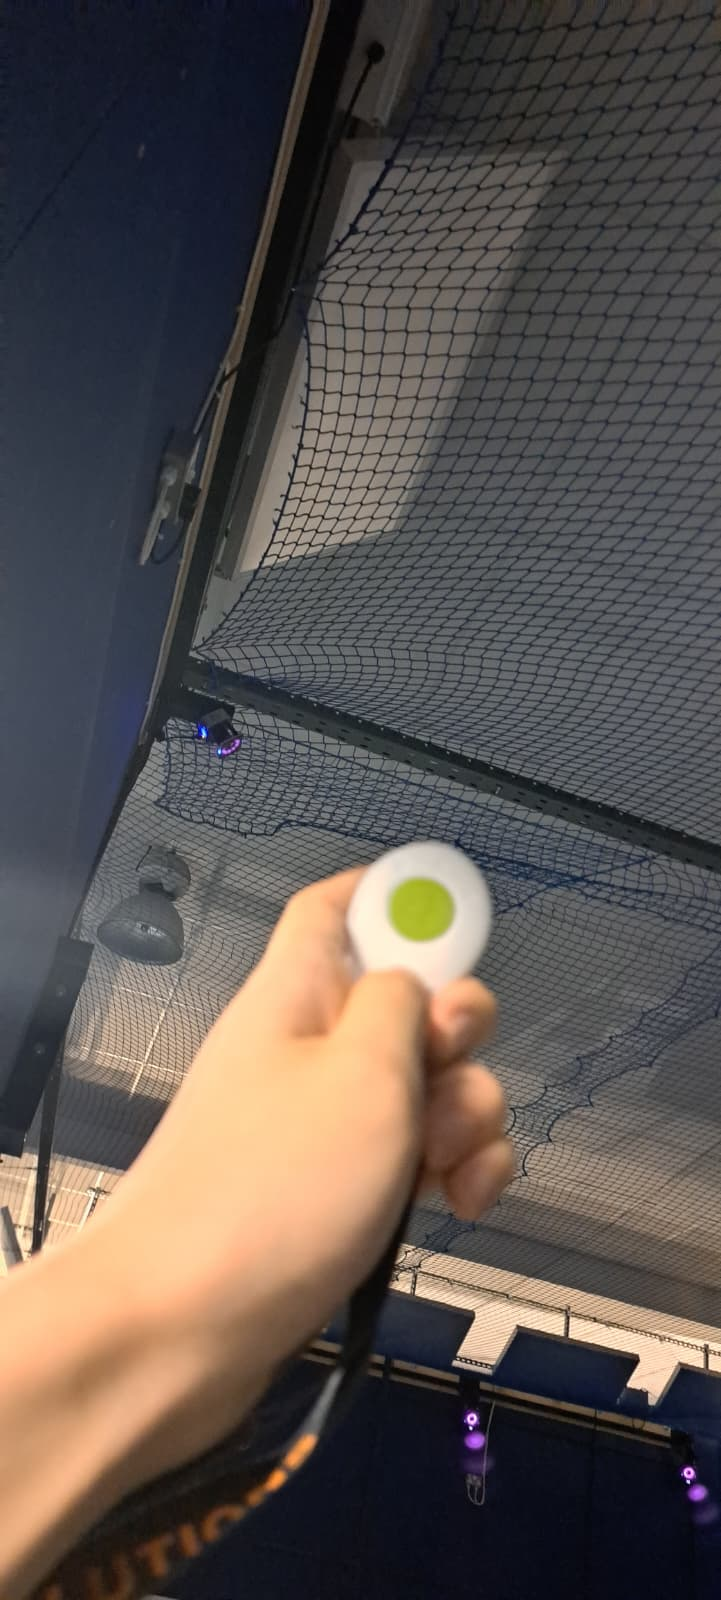
\includegraphics[width=\linewidth]{Images/WhatsApp Image 2026-02-24 at 19.05.02 (2).jpeg}
        \caption{Aim the button towards the celling and depress the button.}
    \end{subfigure}
    \hfill
    \begin{subfigure}[b]{0.32\linewidth}
        \centering
        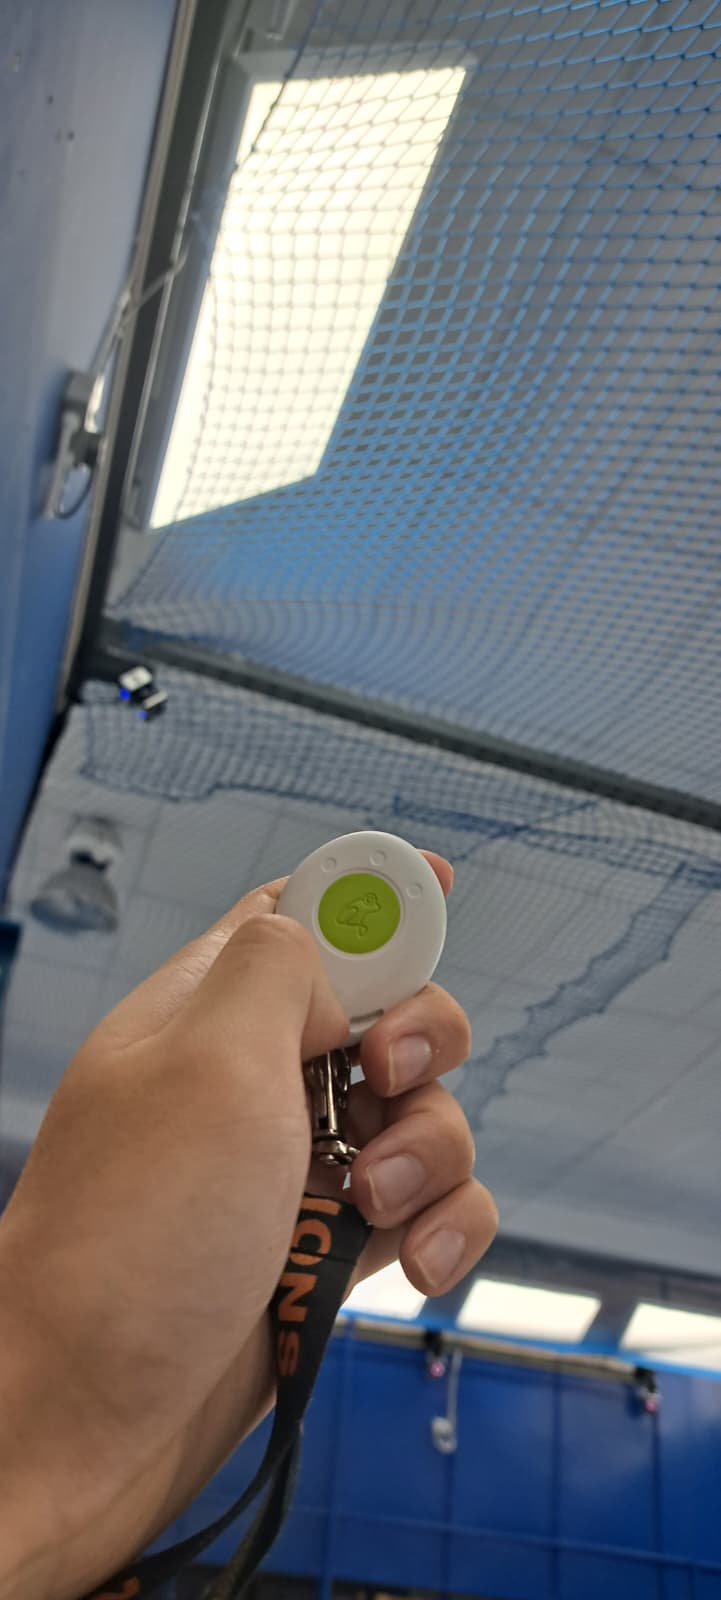
\includegraphics[width=\linewidth]{Images/WhatsApp Image 2026-02-24 at 19.05.02 (3).jpeg}
        \caption{Lights turns on!\\Hooray!}
    \end{subfigure}
    \caption{Image of how to turn on the flight arena lights}
    \label{fig:three_subfigs}
\end{figure}

\subsection{Calibrate the Cameras}
Next, the cameras need to be calibrated. Under the category \textit{CALIBRATE CAMERAS,} seen in figure \ref{fig:9}, click \textit{START}. The computer will verbally respond with "Calibration started". 
\begin{figure}[H]
    \centering
    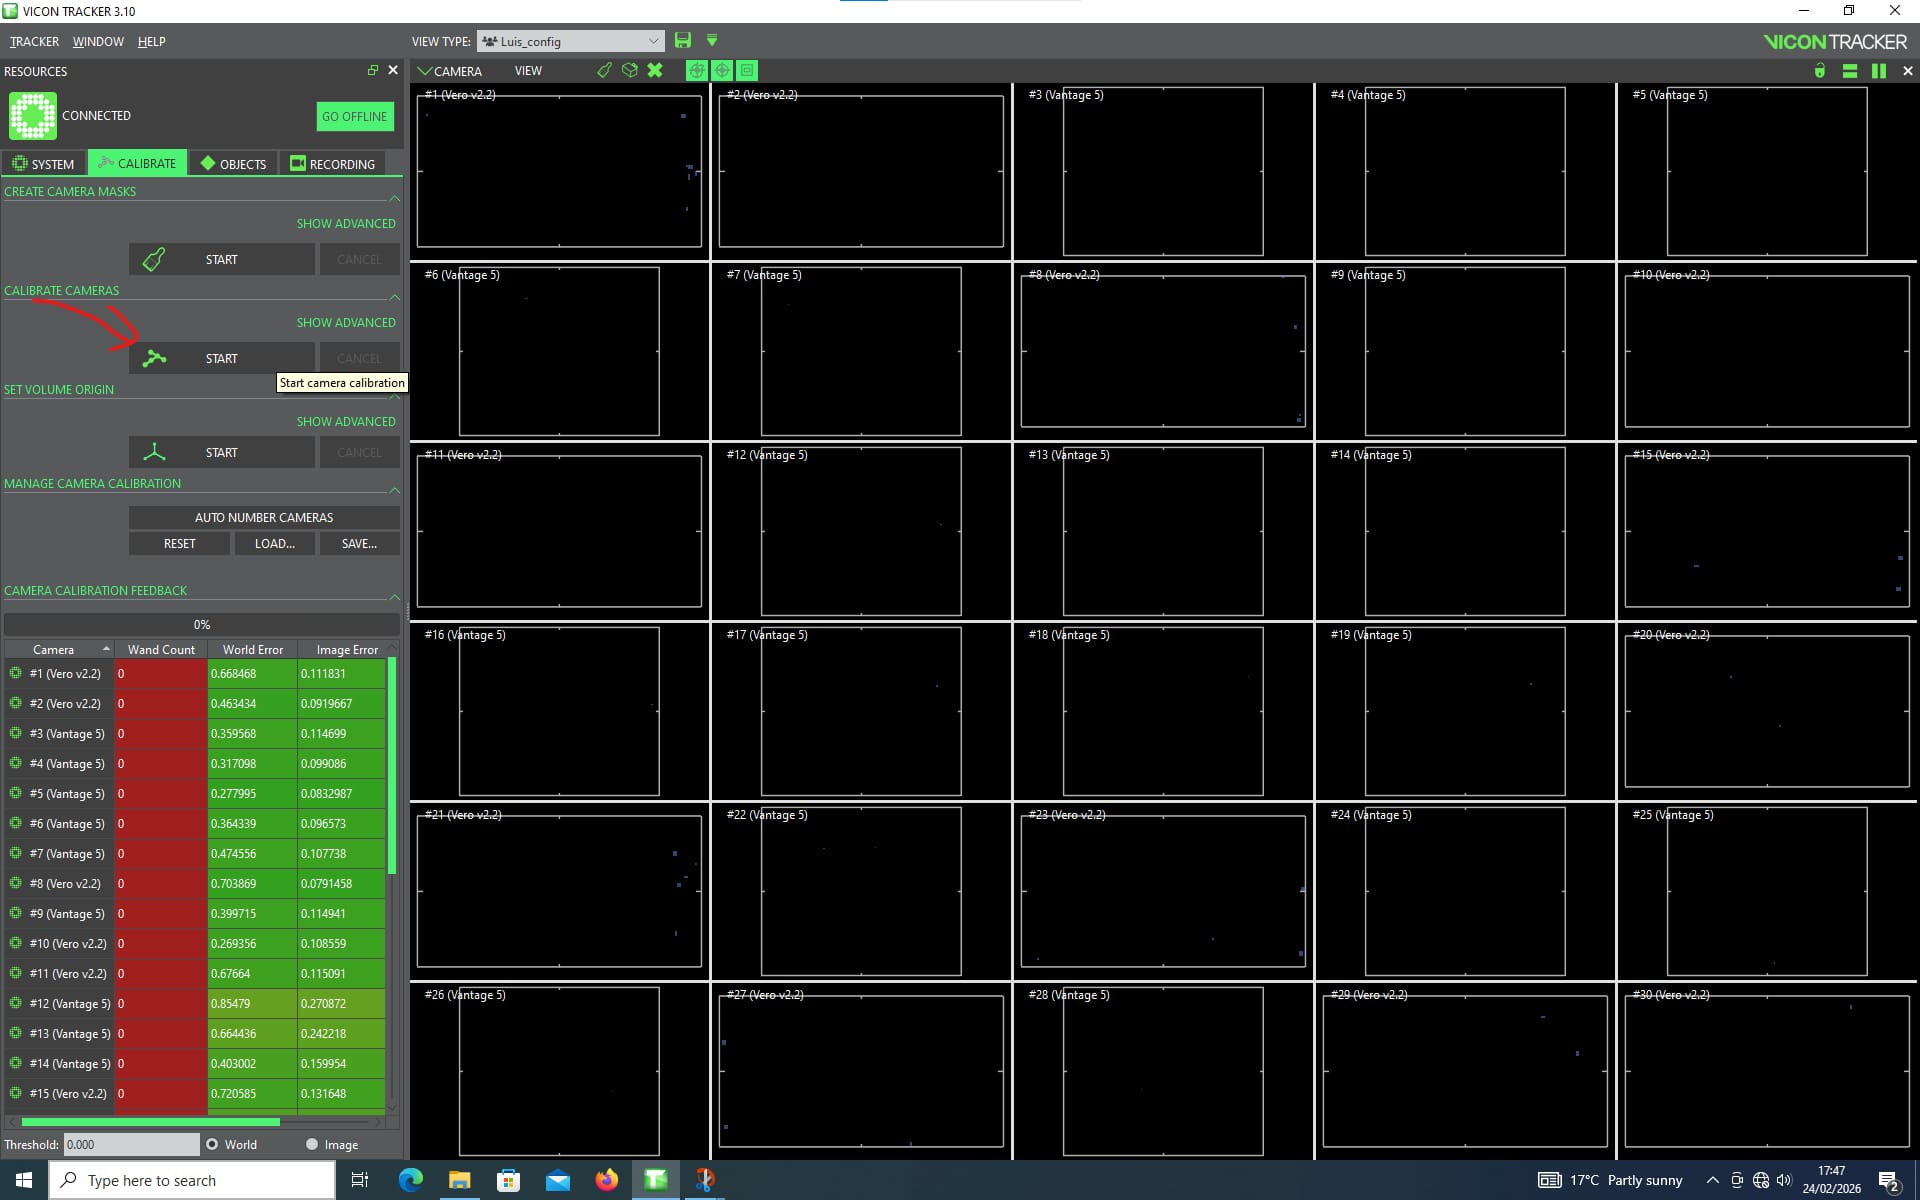
\includegraphics[width=0.8\linewidth]{Images/WhatsApp Image 2026-02-24 at 19.06.17 (3).jpeg}
    \caption{Image of the \textit{CALIBRATION CAMERAS}'s \textit{START} button.}
    \label{fig:9}
\end{figure}





Search for the Vicon Calibration Wand. Find the LED switch as seen in figure \ref{fig:10} and switch it on, red lights should come on. 
\begin{figure}[H]
    \centering
    \begin{subfigure}[b]{0.32\linewidth}
        \centering
        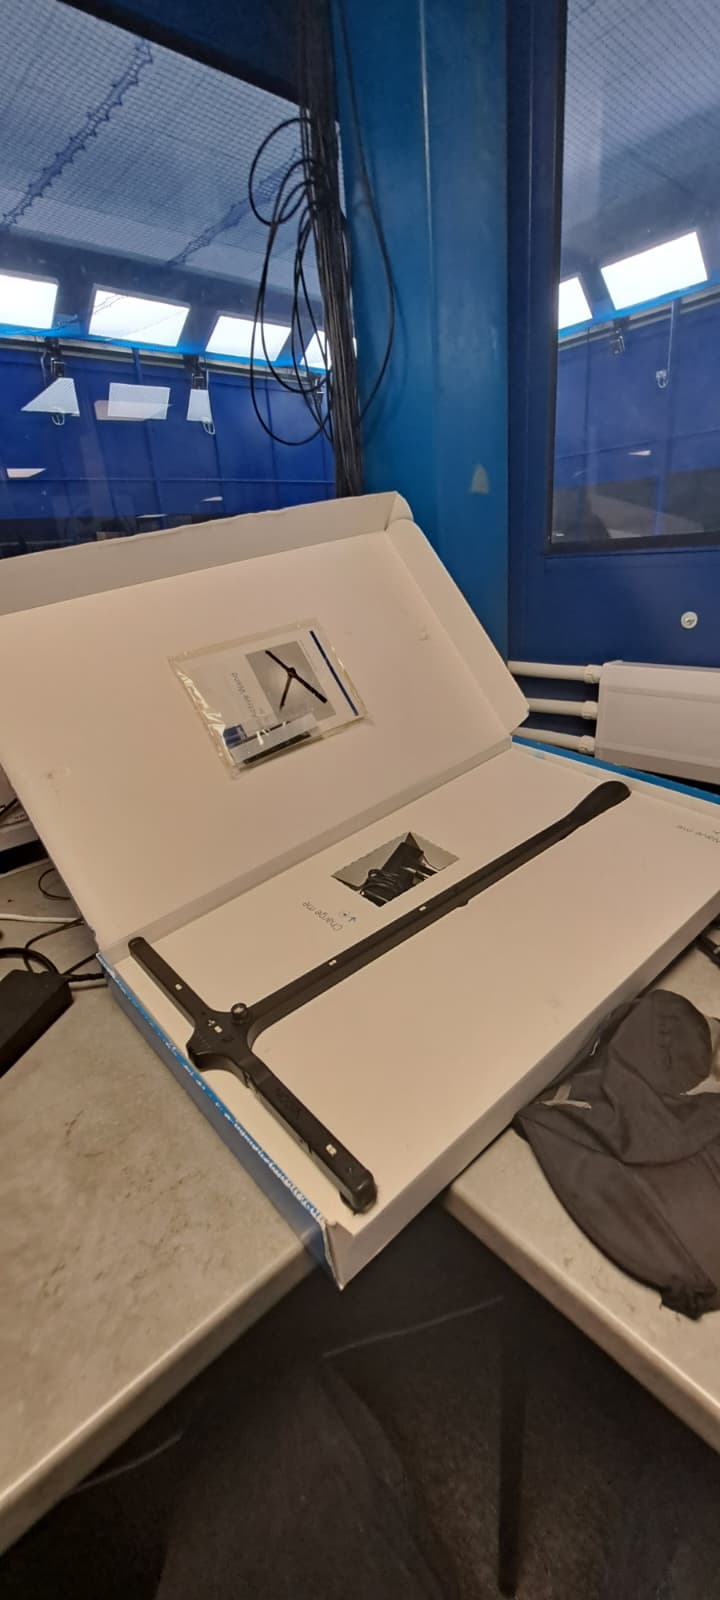
\includegraphics[width=\linewidth]{Images/WhatsApp Image 2026-02-24 at 19.06.18.jpeg}
        \caption{\raggedright The VICON Calibration Wand and its spawn point.}
        \label{fig:sub1}
    \end{subfigure}
    \hfill
    \begin{subfigure}[b]{0.32\linewidth}
        \centering
        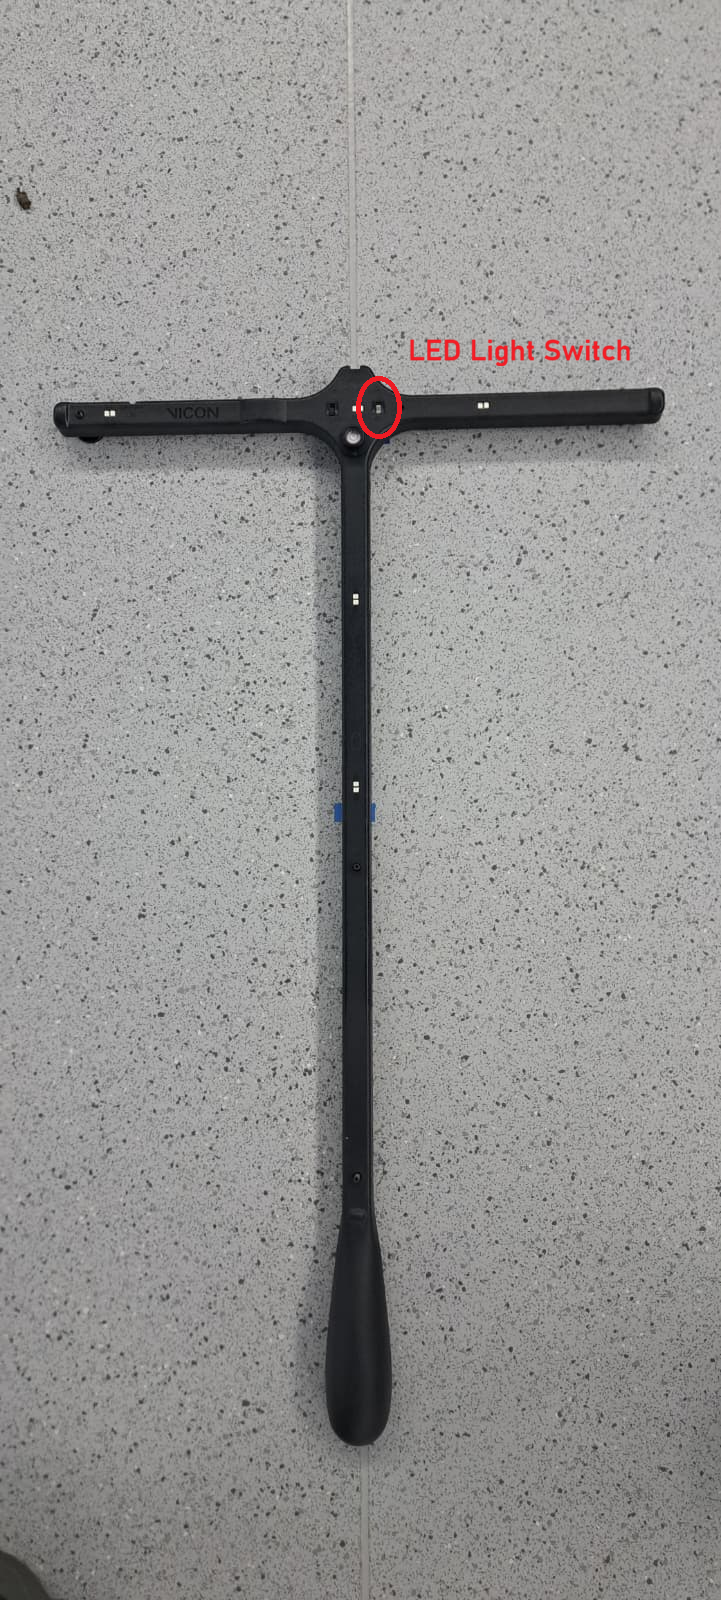
\includegraphics[width=\linewidth]{Images/WhatsApp Image 2026-02-24 at 19.06.11 (2).png}
        \caption{\raggedright The Wand and the LED light switch.}
        \label{fig:sub2}
    \end{subfigure}
    \hfill
    \begin{subfigure}[b]{0.32\linewidth}
        \centering
        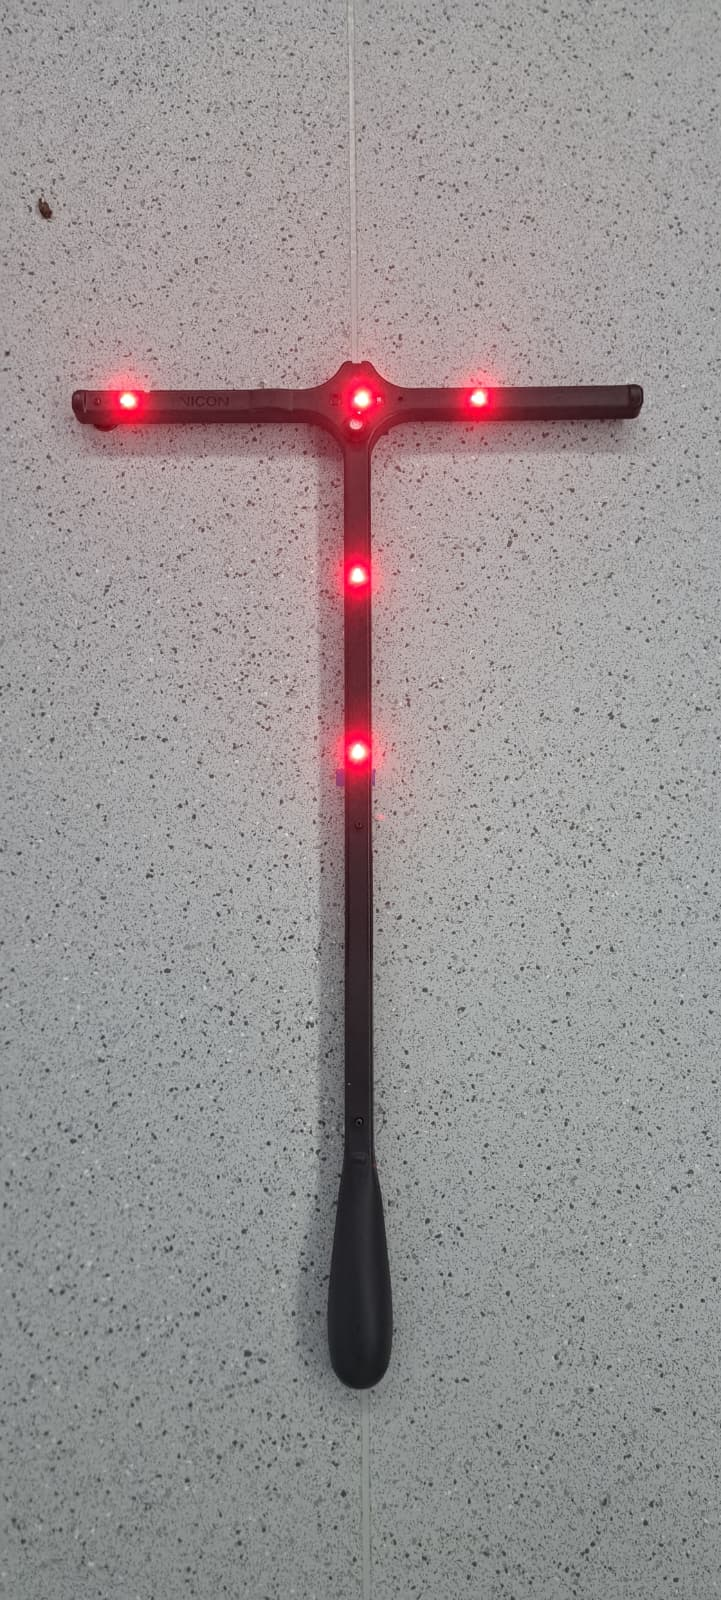
\includegraphics[width=\linewidth]{Images/WhatsApp Image 2026-02-24 at 19.06.12 (1).jpeg}
        \caption{\raggedright Lights turns on! \\ Hooray!}
        \label{fig:sub3}
    \end{subfigure}
    \caption{Image of how to turn on the VICON Calibration Wand}
    \label{fig:10}
\end{figure}

Biomechanically, leave the Host PC and walk into the flight arena and sweep your arm in a cyclical pattern towards the cameras, an example of such interpretive dance can be seen below in figure \ref{fig:5}.
\begin{figure}[H]
    \centering

    % Row 1
    \begin{subfigure}[b]{0.23\linewidth}
        \centering
        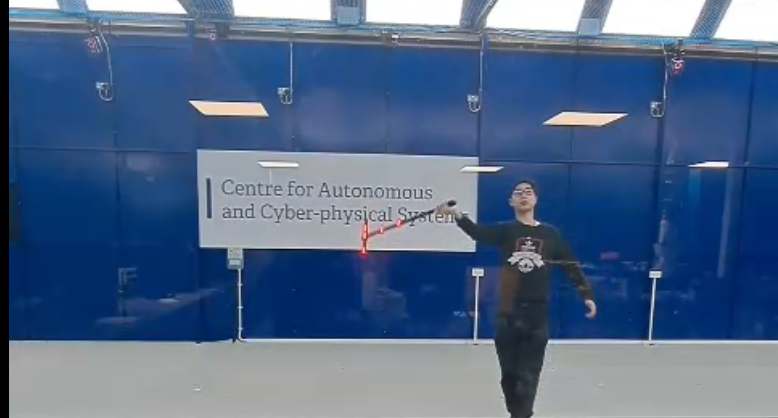
\includegraphics[width=\linewidth]{Images/Dance1.png}
        \label{fig:d1}
    \end{subfigure}
    \hfill
    \begin{subfigure}[b]{0.23\linewidth}
        \centering
        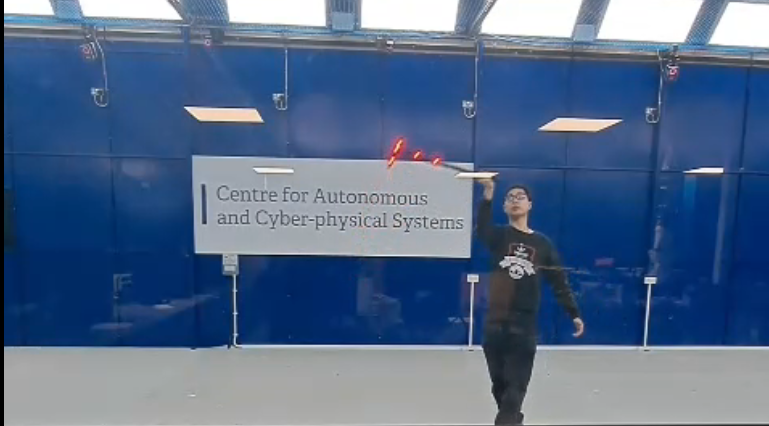
\includegraphics[width=\linewidth]{Images/Dance2.png}
        \label{fig:d2}
    \end{subfigure}
    \hfill
    \begin{subfigure}[b]{0.23\linewidth}
        \centering
        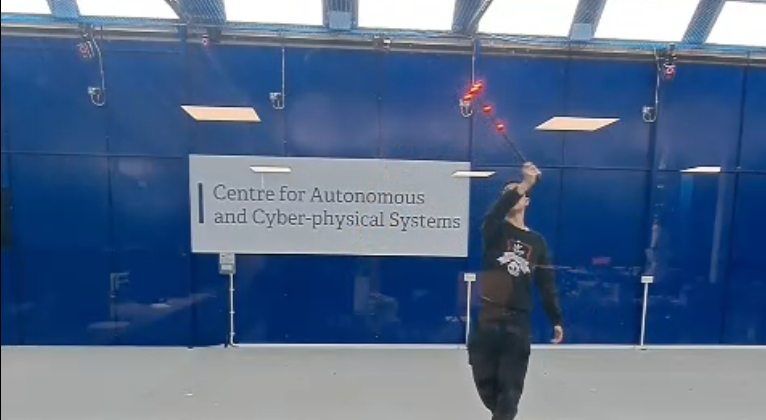
\includegraphics[width=\linewidth]{Images/Dance3.png}
        \label{fig:d3}
    \end{subfigure}
    \hfill
    \begin{subfigure}[b]{0.23\linewidth}
        \centering
        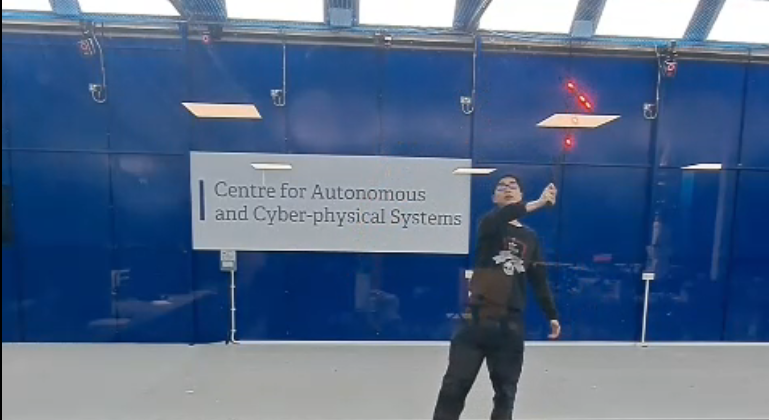
\includegraphics[width=\linewidth]{Images/Dance4.png}
        \label{fig:d4}
    \end{subfigure}

    \vspace{0.5em}

    % Row 2
    \begin{subfigure}[b]{0.23\linewidth}
        \centering
        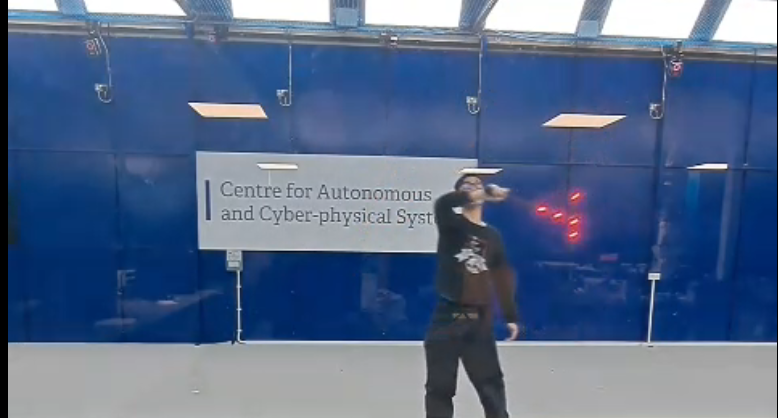
\includegraphics[width=\linewidth]{Images/Dance5.png}
        \label{fig:d5}
    \end{subfigure}
    \hfill
    \begin{subfigure}[b]{0.23\linewidth}
        \centering
        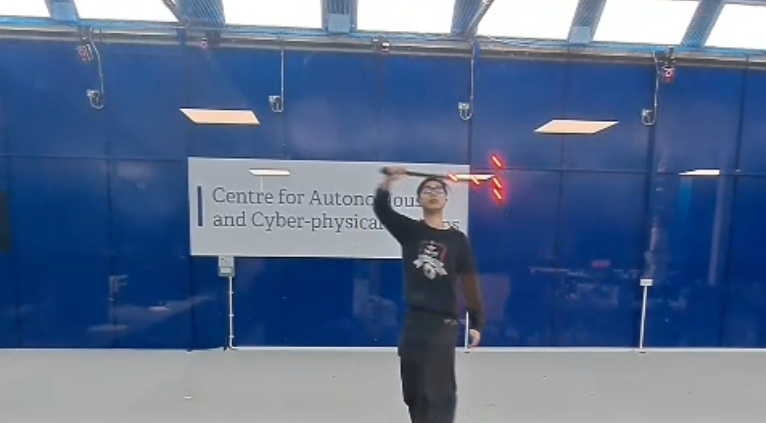
\includegraphics[width=\linewidth]{Images/Dance6.png}
        \label{fig:d6}
    \end{subfigure}
    \hfill
    \begin{subfigure}[b]{0.23\linewidth}
        \centering
        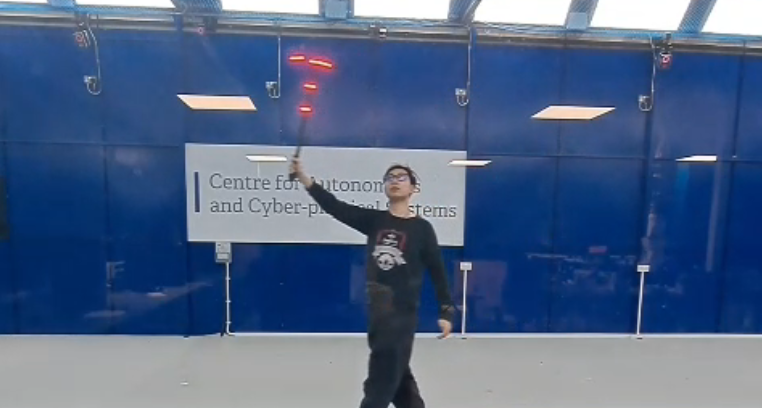
\includegraphics[width=\linewidth]{Images/Dance7.png}
        \label{fig:d7}
    \end{subfigure}
    \hfill
    \begin{subfigure}[b]{0.23\linewidth}
        \centering
        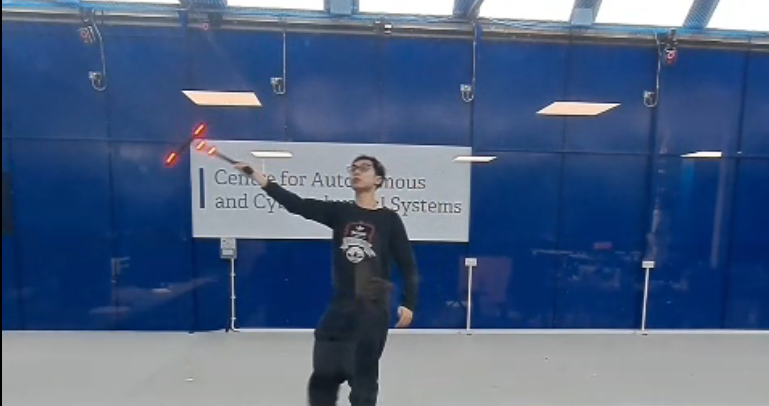
\includegraphics[width=\linewidth]{Images/Dance8.png}
        \label{fig:d8}
    \end{subfigure}

    \caption{Images of dance moves used calibrate the cameras.}
    \label{fig:dance_all}
\end{figure}

Repeat this sweeping motion in front of all the cameras within the flight arena. To determine if a specific camera has been calibrated (or when you can stop sweeping in front of it), you can visually see the LED changes from red/pink to green for the small cameras, and red to green for the big cameras. (For big cameras, you can see a screen on the camera that shows the progress bar of the calibration, see figure \ref{fig:12}). Repeat your interpretive dance until all cameras are calibrated. Visually, all camera would turn from static green to static red if every camera is calibrated. 

\begin{figure}[H]
    \centering
    \begin{subfigure}[b]{0.23\linewidth}
        \centering
        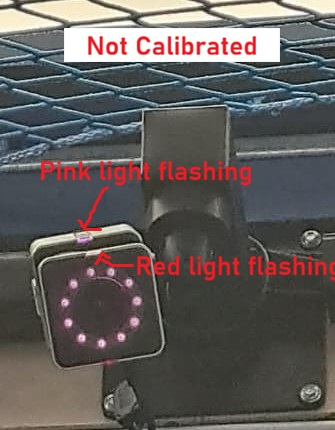
\includegraphics[width=\linewidth]{Images/Small Camera light on.jpeg}
    \end{subfigure}
    \begin{subfigure}[b]{0.23\linewidth}
        \centering
        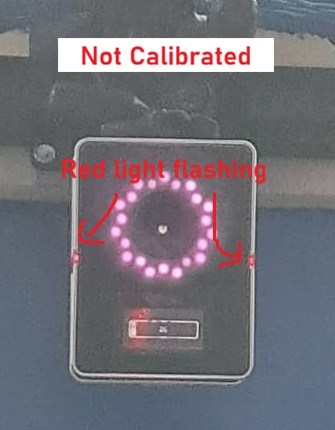
\includegraphics[width=\linewidth]{Images/Big Camera light on.jpeg}
    \end{subfigure}
    \begin{subfigure}[b]{0.23\linewidth}
        \centering
        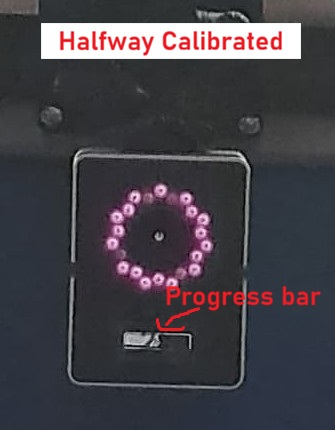
\includegraphics[width=\linewidth]{Images/Big Camera calibrating.jpeg}
    \end{subfigure}
    \begin{subfigure}[b]{0.23\linewidth}
        \centering
        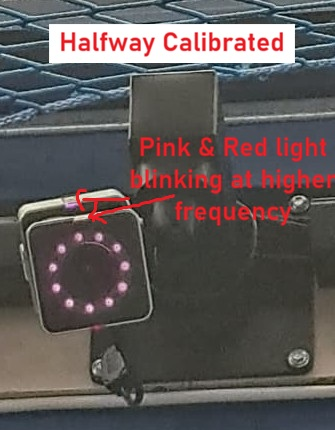
\includegraphics[width=\linewidth]{Images/Small Camera calibrating.jpeg}
    \end{subfigure}
    \hfill
     \vspace{0.5em}
     \begin{subfigure}[b]{0.23\linewidth}
        \centering
        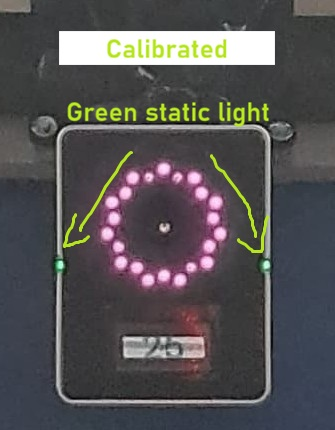
\includegraphics[width=\linewidth]{Images/Big Camera Calibrated.jpeg}
    \end{subfigure}
    \begin{subfigure}[b]{0.23\linewidth}
        \centering
        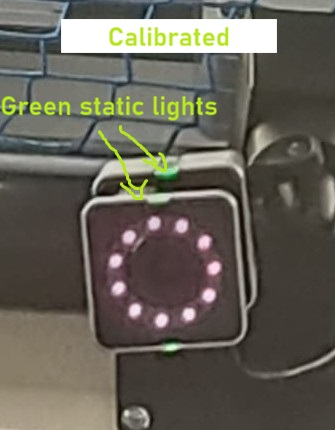
\includegraphics[width=\linewidth]{Images/Small Camera Calibrated.jpeg}
    \end{subfigure}
    \hfill
    \caption{Images of camera stage's of calibration and it's visual indicators.}
    \label{fig:12}
\end{figure}
\clearpage
Return to the PC, focus on the bottom left of your screen on \textit{CAMERA CALIBRATION FEEDBACK}, a progress bar will show the calculation of the poses from the Tracker, shown in figure \ref{fig:13} below. 
\begin{figure}[H]
    \centering
    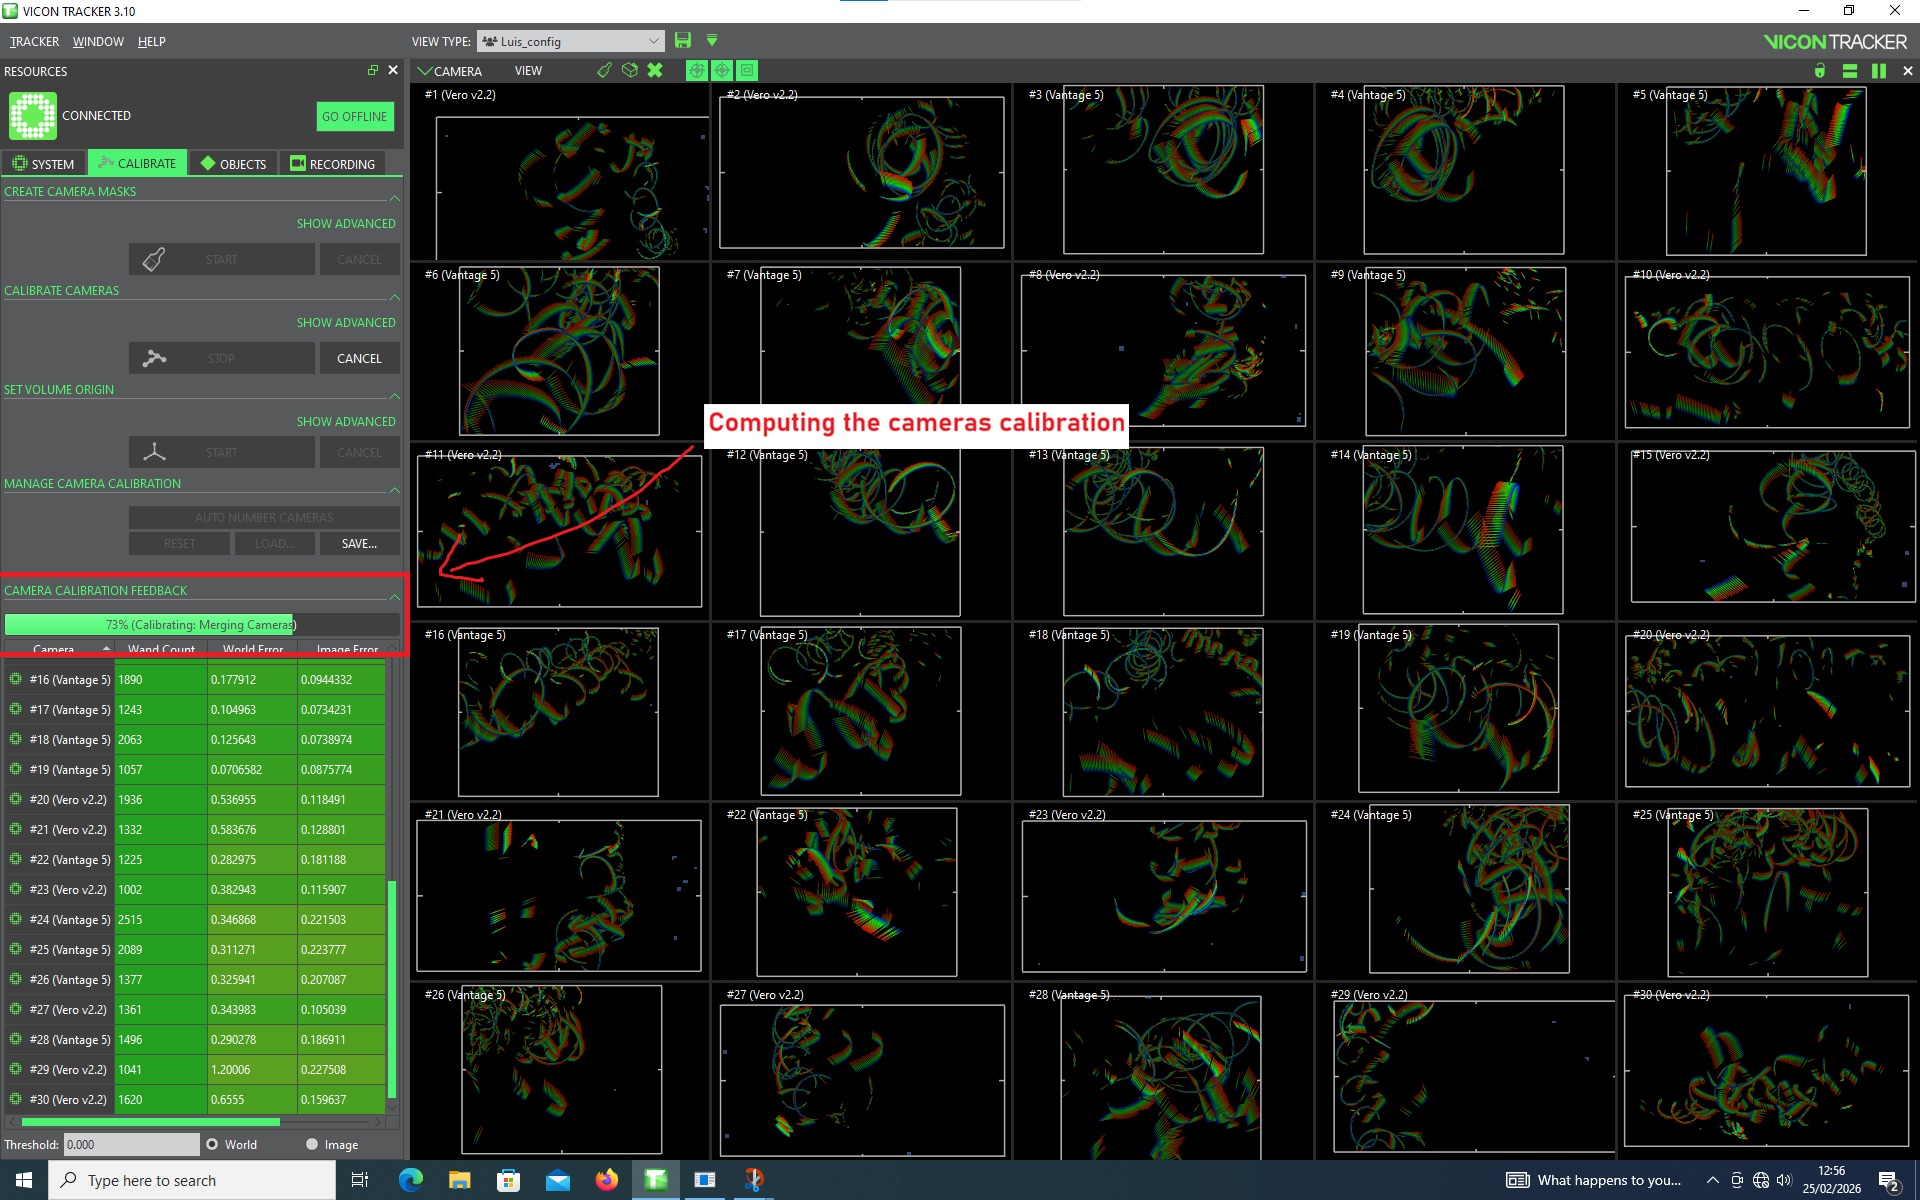
\includegraphics[width=1\linewidth]{Images/8.75 Calibrating Camera.png}
    \caption{Image of feedback computation after physical camera calibration}
    \label{fig:13}
\end{figure}


Once the calculation progress bar is filled and therefore completed, check the \textit{World Error} and \textit{Image Error} from all the cameras, If you see any orange or red tiles from the table as shown in figure \ref{fig:14}, you will need to repeat your calibration step.
\begin{figure}[H]
    \centering
    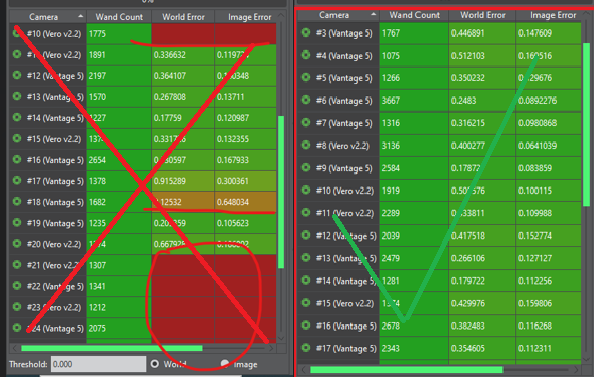
\includegraphics[width=0.8\linewidth]{Images/Bad vs good camera calibration.png}
    \caption{Comparison figure of bad vs good camera calibration}
    \label{fig:14}
\end{figure}
\subsection{Set Origin}
Next, you will need to set the origin of your coordinate system. This essentially defines your x y z axis for your inertial positioning system. Without pressing anything on the PC, physically go back into the flight arena with the Vicon Calibration Wand. Place your wand flat on the ground on where you want to defined your origins are. 

For default, I suggest you place them on the blue tapes in the intersectional middle of the flight arena, as seen in figure \ref{fig:31}
\begin{figure}[H]
    \centering

    \begin{subfigure}[b]{0.32\linewidth}
        \centering
        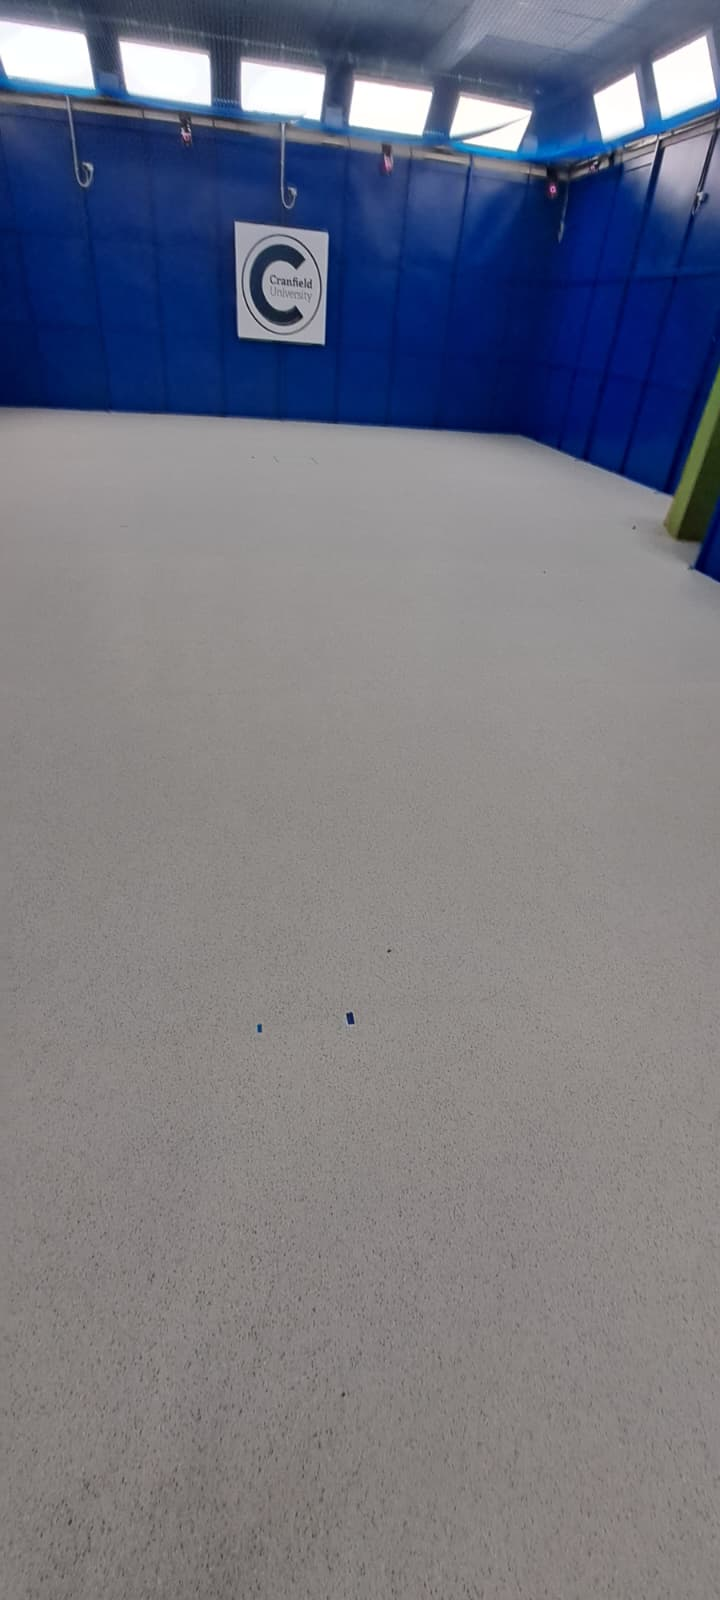
\includegraphics[width=\linewidth]{Images/WhatsApp Image 2026-02-24 at 19.06.11.jpeg}
        \caption{\raggedright Default location for origin, located in the middle intersectional area.}
    \end{subfigure}
    \hfill
    \begin{subfigure}[b]{0.32\linewidth}
        \centering
        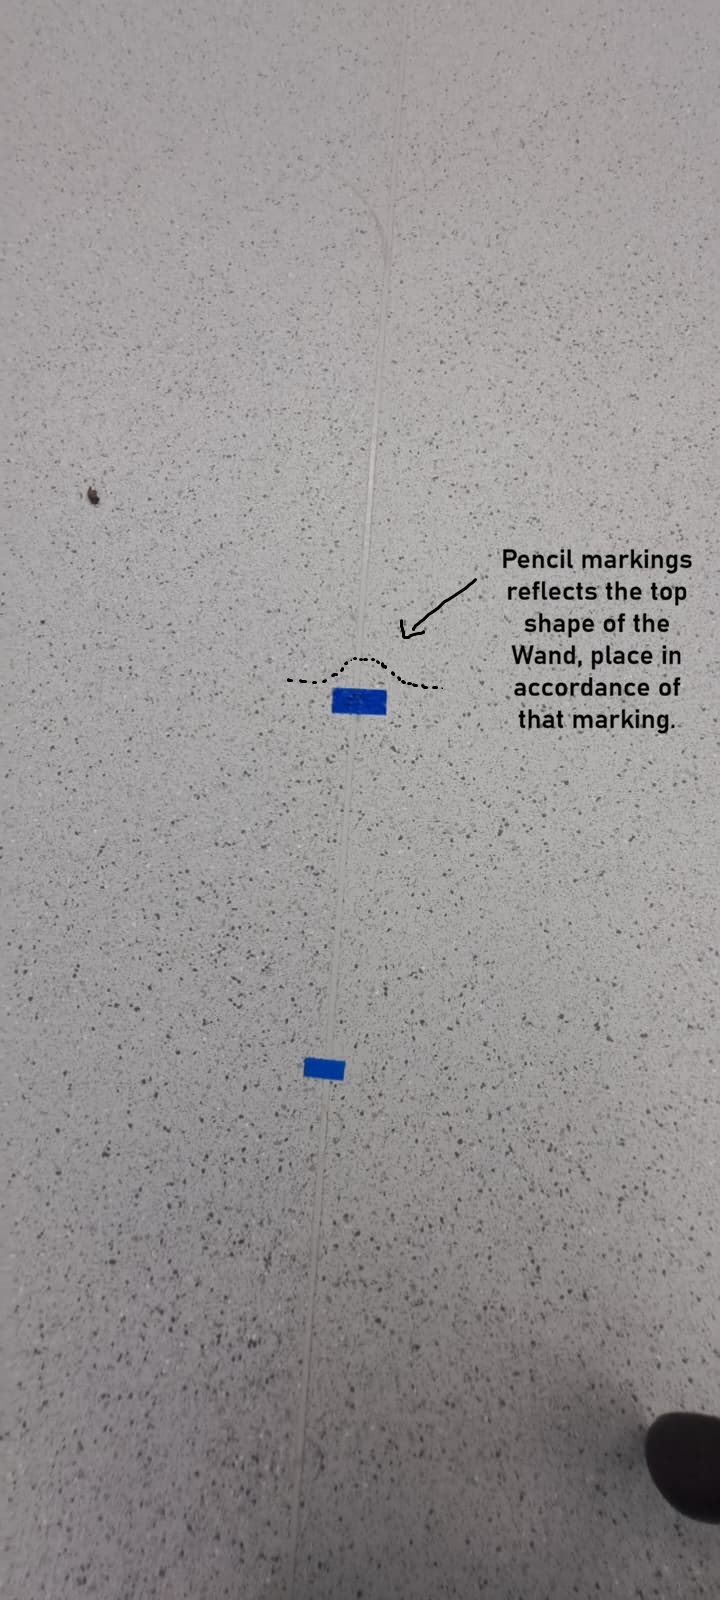
\includegraphics[width=\linewidth]{Images/WhatsApp Image 2026-02-24 at 19.06.09.jpeg}
        \caption{\raggedright Closed up location, identifiable with 2 blue tapes and pencil markings.}
    \end{subfigure}
    \hfill
    \begin{subfigure}[b]{0.32\linewidth}
        \centering
        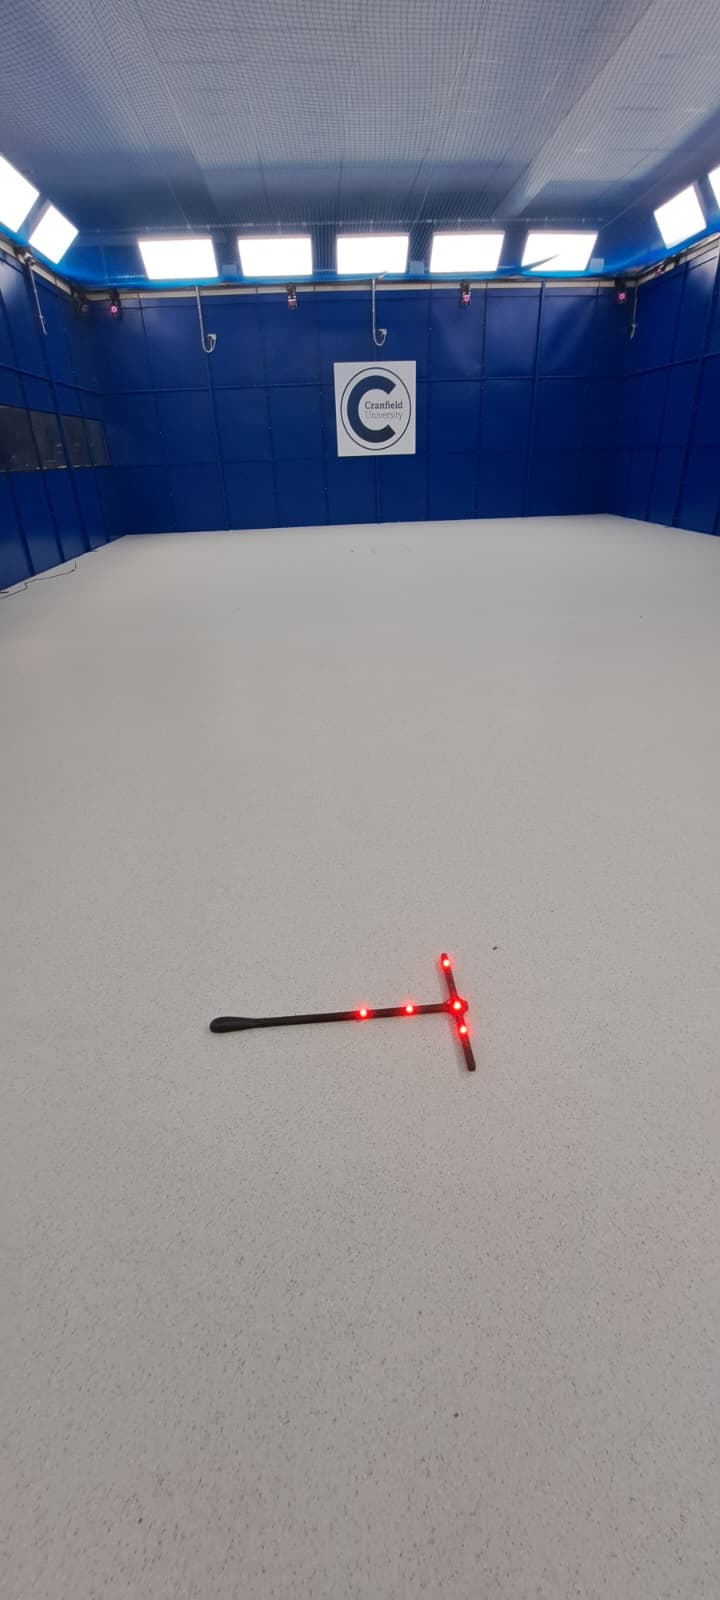
\includegraphics[width=\linewidth]{Images/WhatsApp Image 2026-02-24 at 19.06.12 (2).jpeg}
        \caption{\raggedright Overall wand placement location for origin. Located in the corner of flight arena.\\
        }
    \end{subfigure}
    \caption{Conventional origin location placement for Vicon Calibration Wand.}
    \label{fig:31}
\end{figure}

Noting that the direction convention for the Vicon Calibration Wand is that bottom of handle faces West, left handle faces North (Refer to figure \ref{fig:16}). With the best of your ability, align it to the orthogonal landscape of the flight arena (The silicone sealant on the floor is a good orthogonal reference, align the wand with it). This is imperative as your Vicon Calibration Wand's West is what the Ardupilot/flight controller determines as it's environment West. If your West is badly oriented, you will just have a non-orthogonal axis as your inertial coordinate frame, for which, your path-planning person will sure thank you a lot for :). 
\begin{figure}[H]
    \centering
    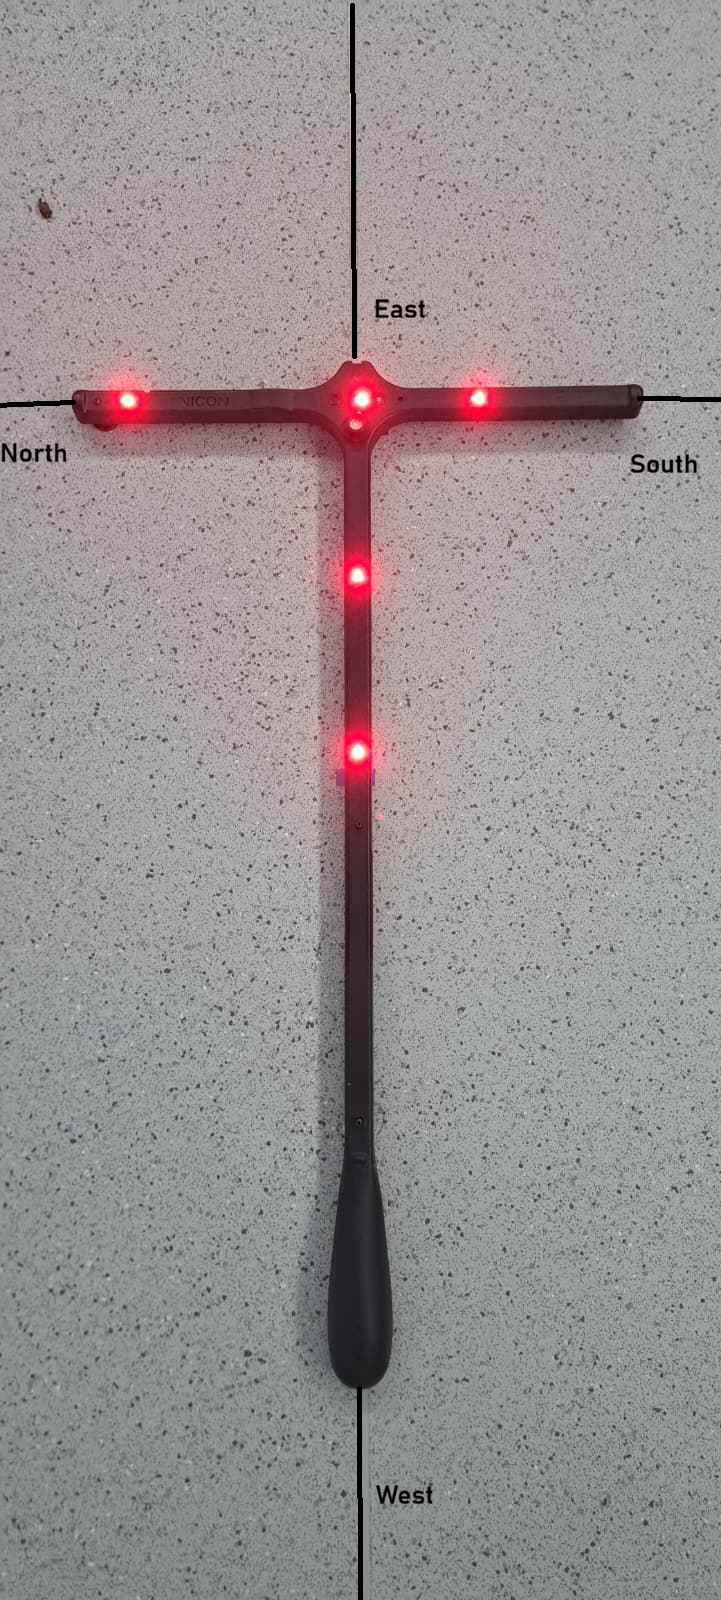
\includegraphics[width=0.5\linewidth]{Images/Direction convention of Vicon Calibration Wand.png}
    \caption{Direction conventions for the Vicon Calibration Wand.}
    \label{fig:16}
\end{figure}
Leave the wand on the ground, return to the PC and navigation to the \textit{SET VOLUME ORIGIN}, click \textit{START} (figure \ref{fig:17}), the computer will respond verbally with "Origin set". 
\begin{figure}[H]
    \centering
    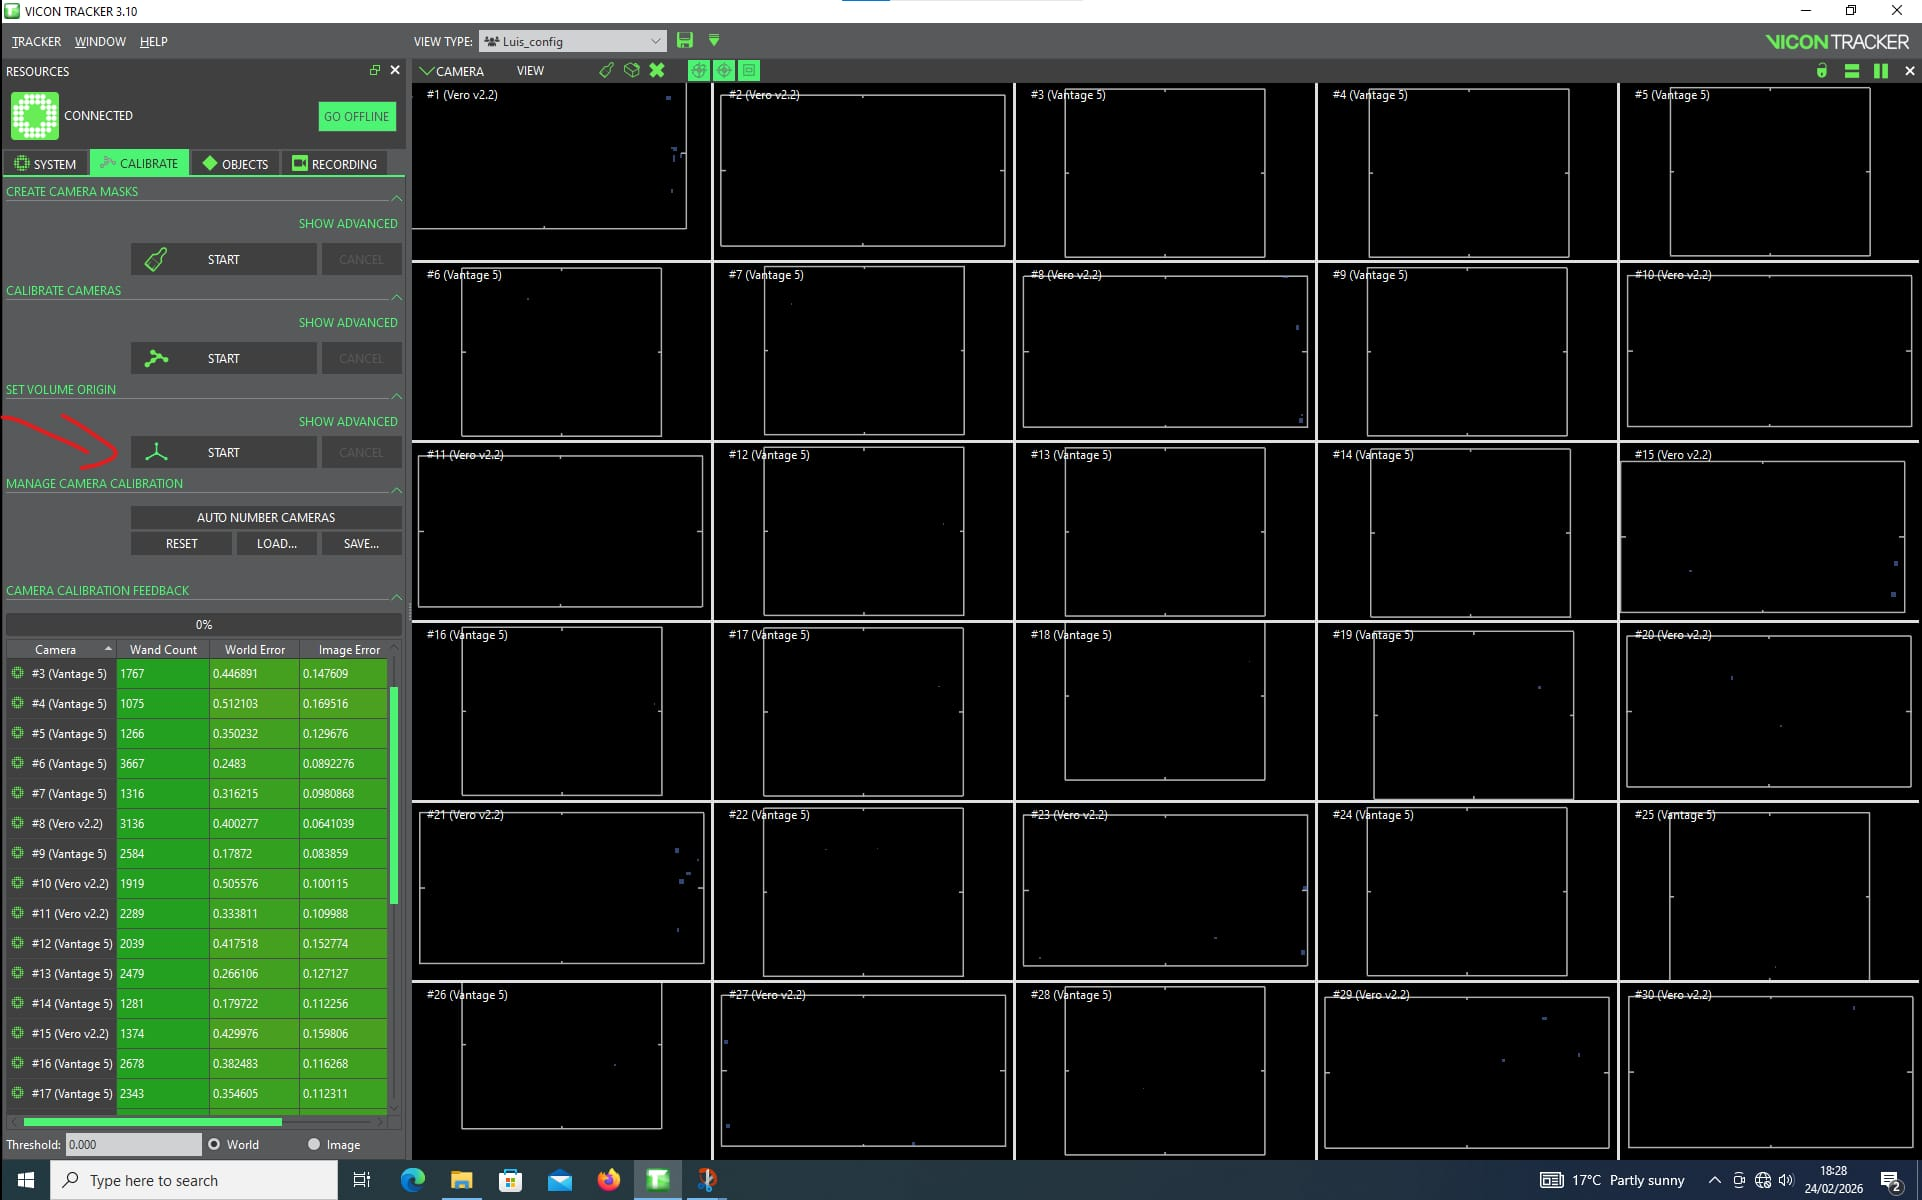
\includegraphics[width=1\linewidth]{Images/WhatsApp Image 2026-02-24 at 19.06.19 (1).jpeg}
    \caption{Image of Set Volume Origin button's location.}
    \label{fig:17}
\end{figure}
\subsection{Defining New Objects}
\label{sec:defineNewObject}
The way objects are recognized in the VICON algorithm is that it remembers the assortment of reflective markers placed on your drone. This works by defining your markers as \textit{Object}. \footnote{For my lovely GDP group, our drone is already defined as an object by yours truly and is called INSP!} 

To make a new Object, you first need to glue the IR markers on your drone (4+ markers as a minimum empirical requirement). An example of which is seen below in figure \ref{fig:18}. 

\begin{figure}[H]
    \centering
    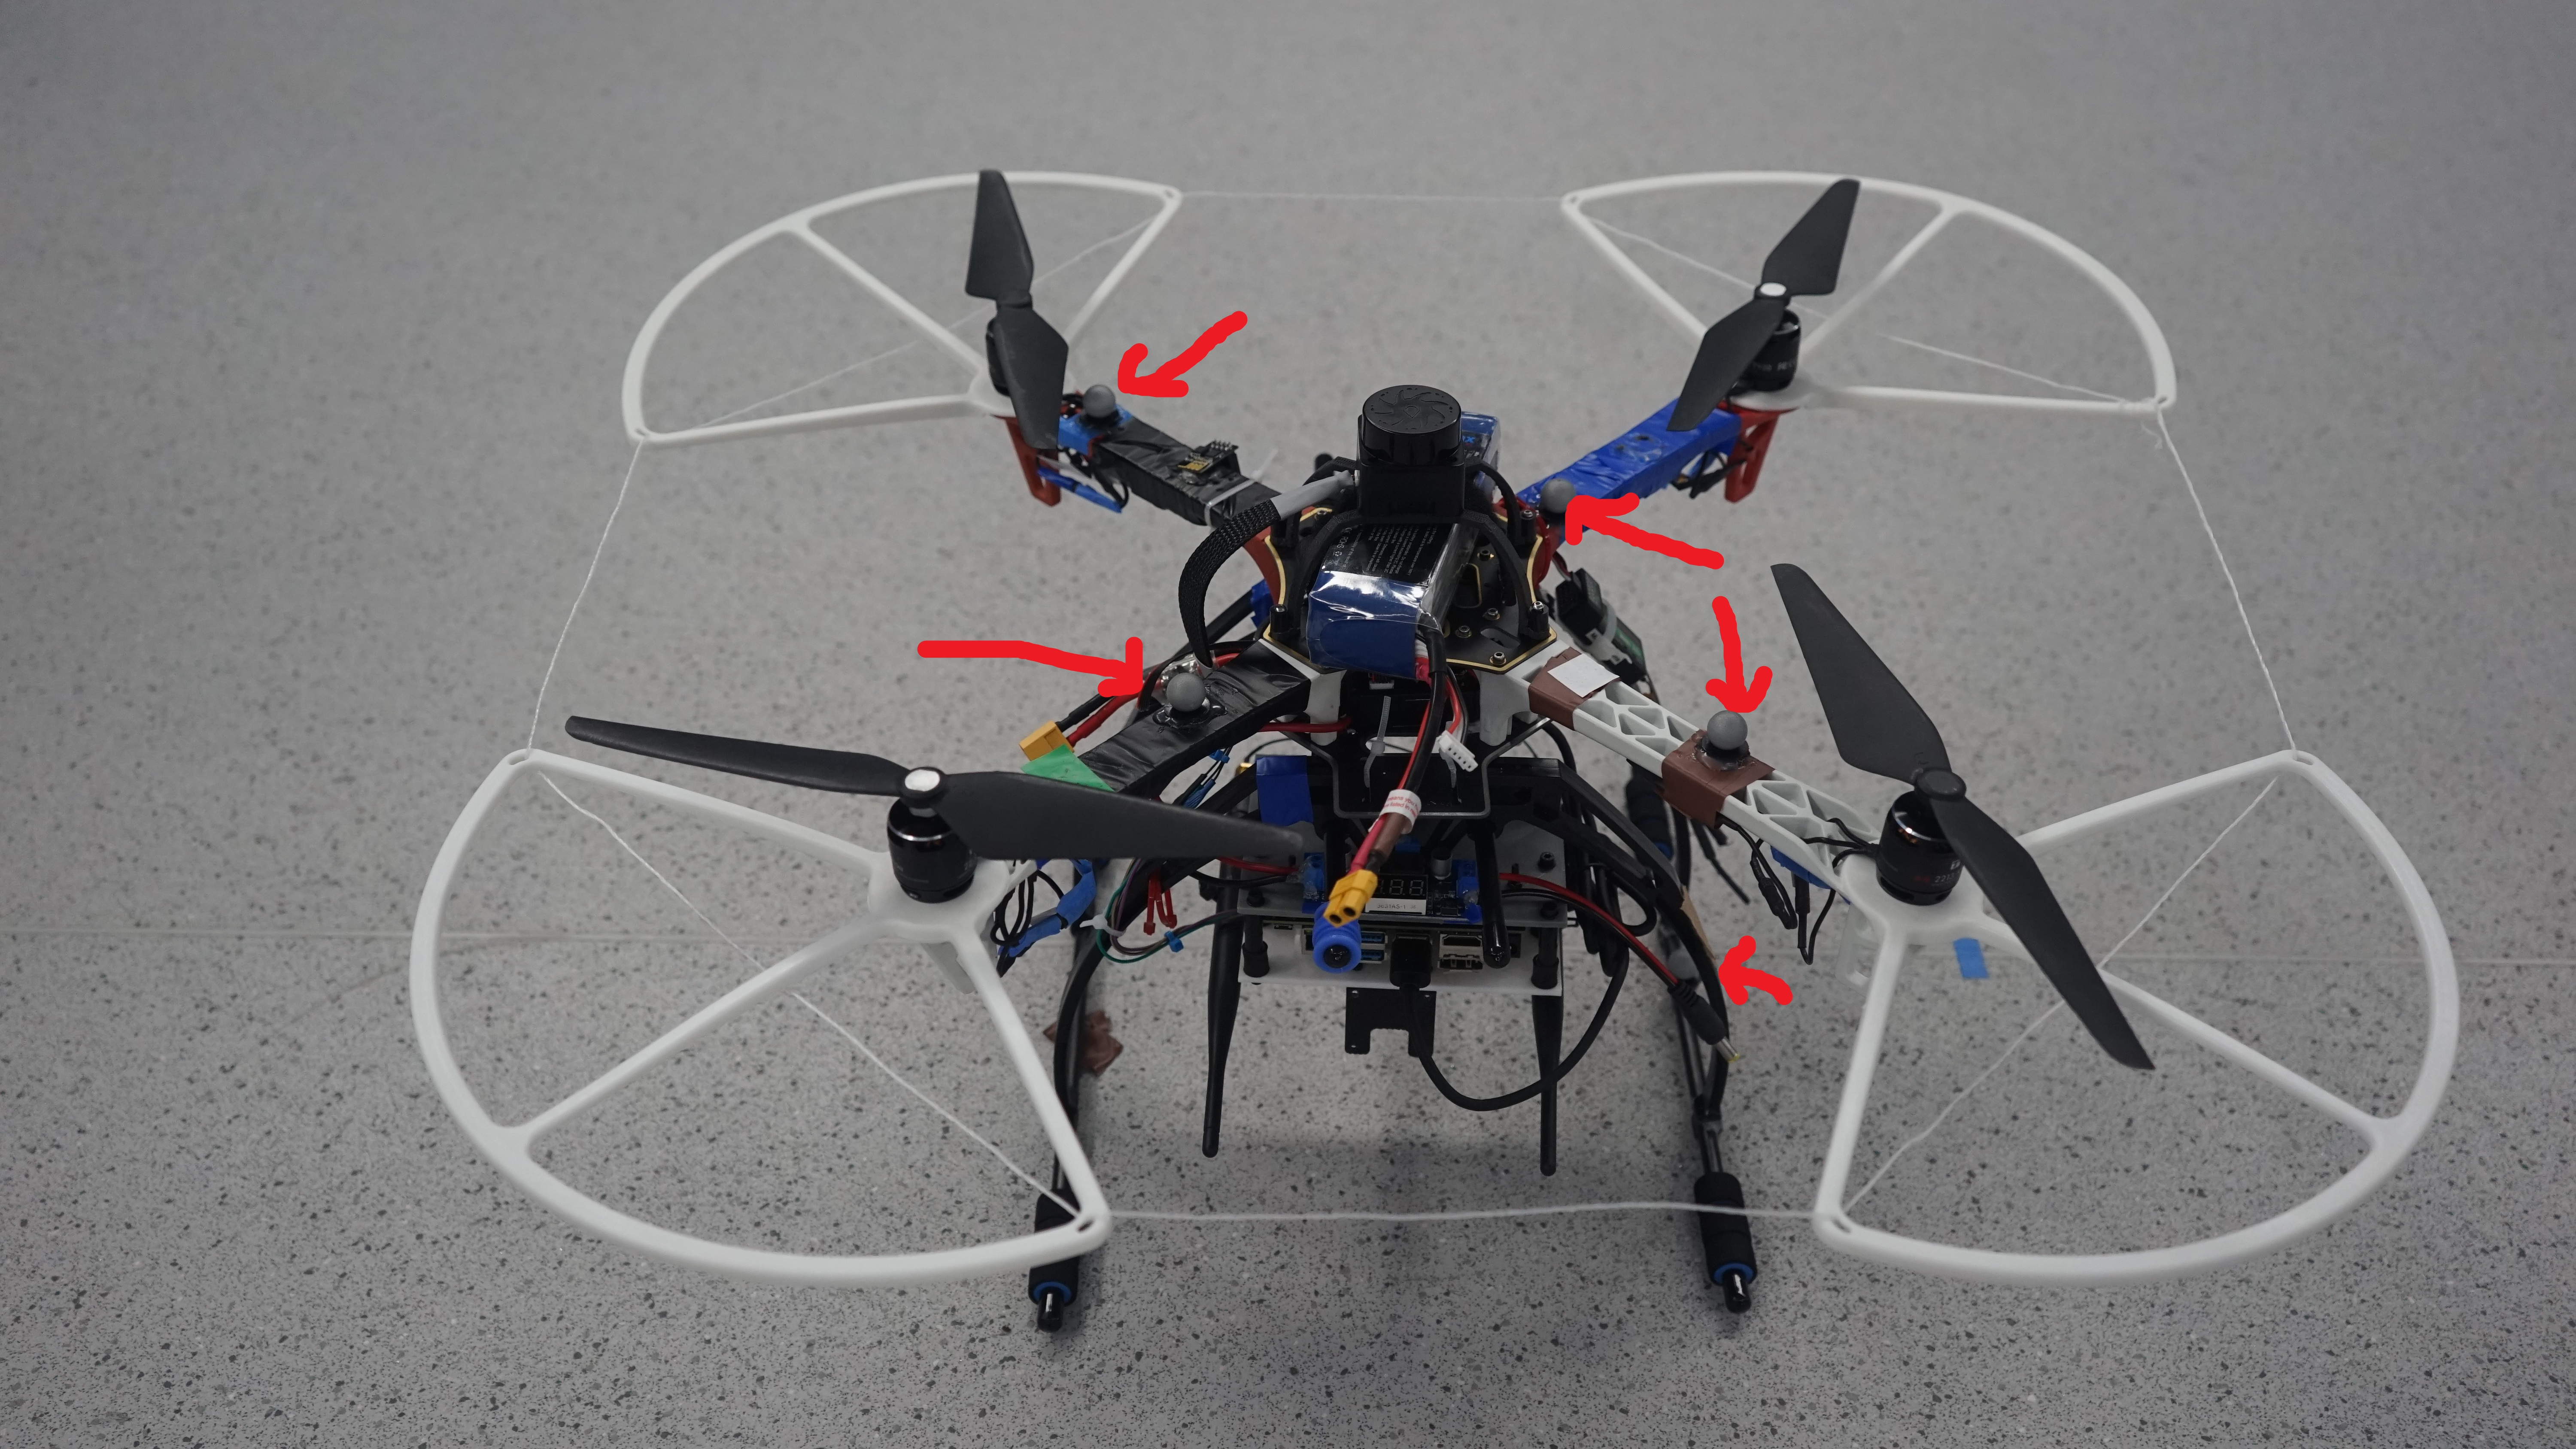
\includegraphics[width=0.8\linewidth]{Images/DSC05445.JPG}
    \caption{Example Image of IR Markers Placement}
    \label{fig:18}
\end{figure}

Once this is done, physically put your drone into the flight arena. Align the front (North) of your drone to the origin's North. Pick up your wand and return to the host PC. 
\begin{figure}[H]
    \centering
    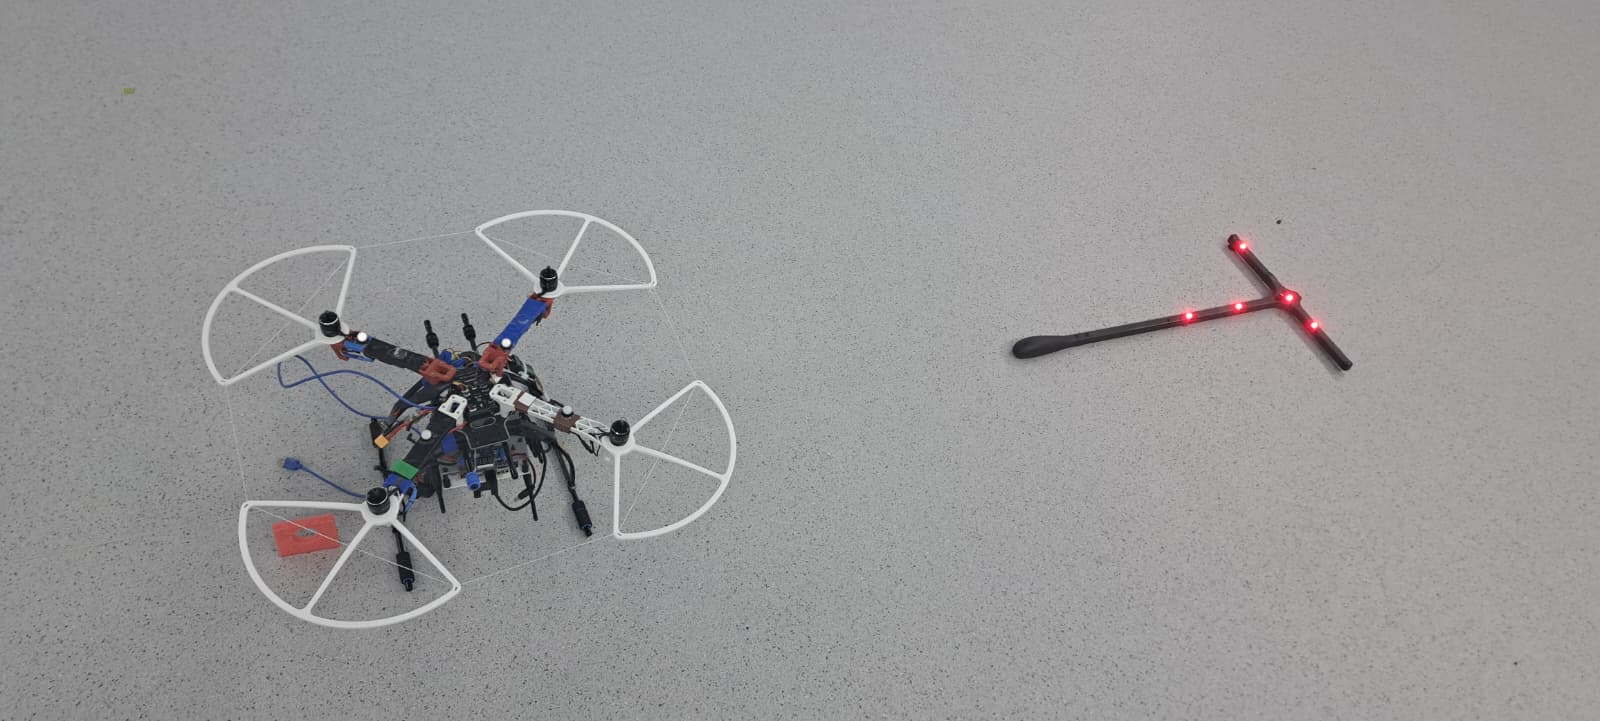
\includegraphics[width=1\linewidth]{Images/WhatsApp Image 2026-02-24 at 19.06.13 (2).jpeg}
    \caption{Image of drone with the Vicon Calibration Wand in it's origin setting position.}
\end{figure}


On the PC's viewport, click the \textit{OBJECT} tab. (If you are in my GDP group, select INSP as the the drone. 
\begin{figure}[H]
    \centering
    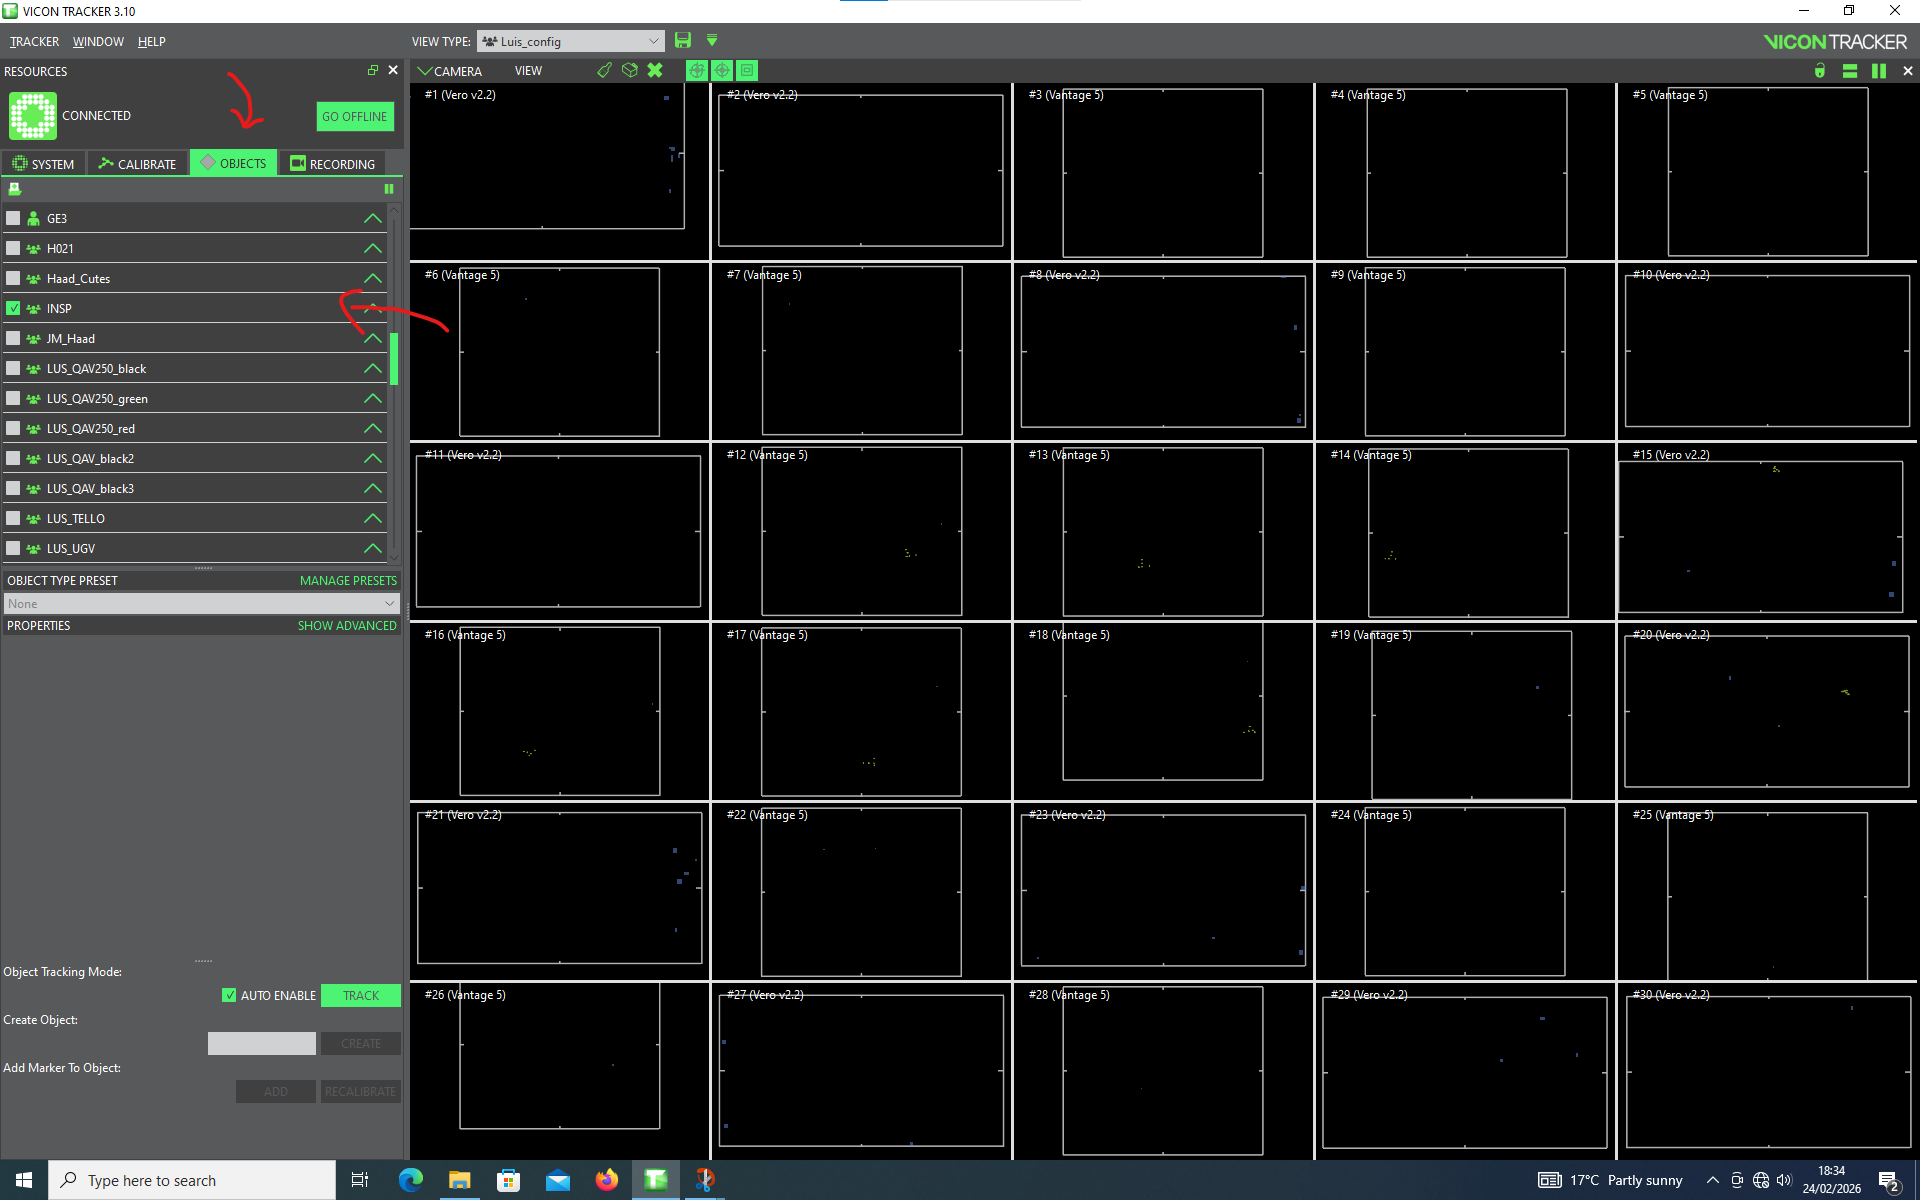
\includegraphics[width=1\linewidth]{Images/11 Objects and selecting objects.png}
    \caption{Enter Caption}
\end{figure}

You need to select the markers in the view port on the right side of the screen. (If you can't see the markers, navigation top left of the view port, and choose \textit{3D ORTHOGONAL} to \textit{-Z}, as seen in figure \ref{fig:20})  

\begin{figure}[H]
    \centering
    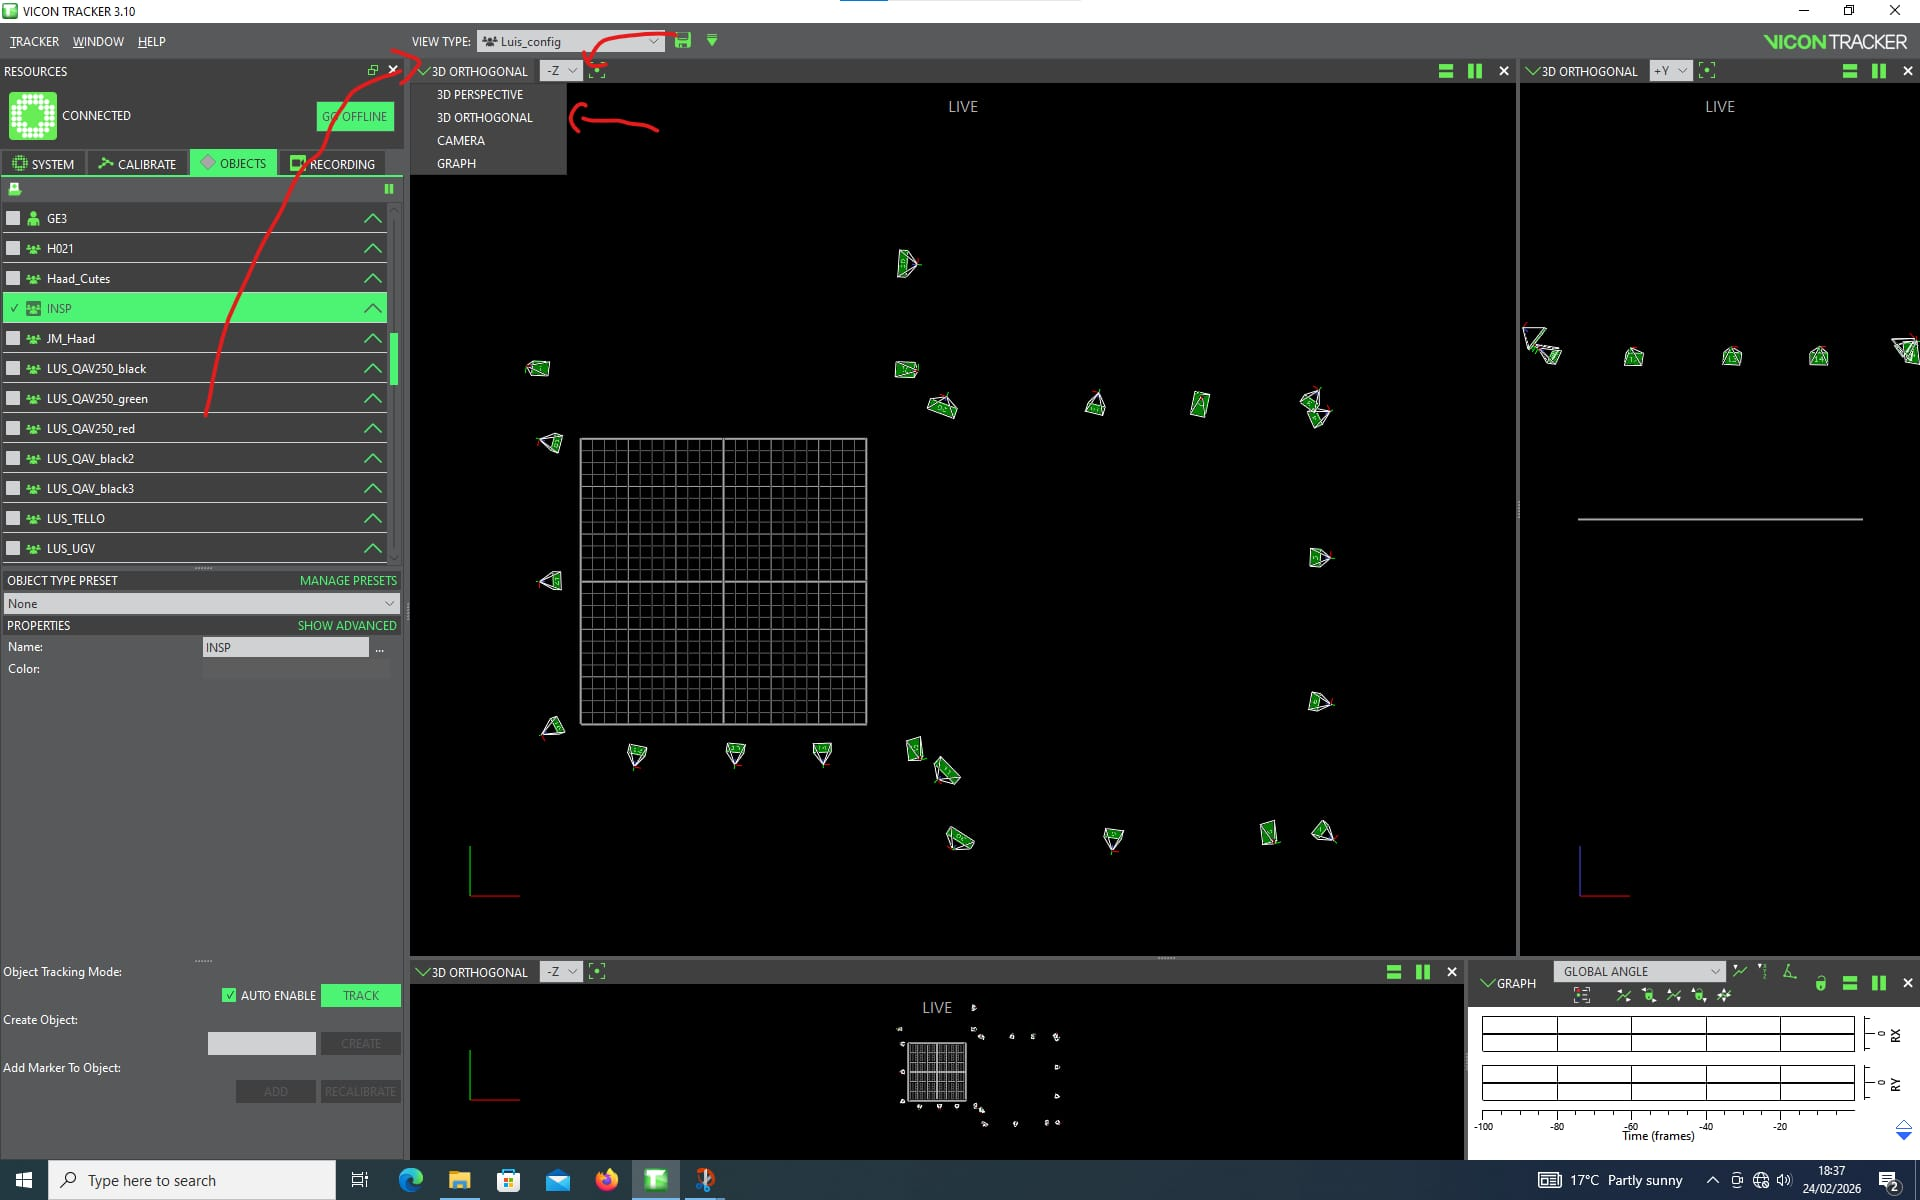
\includegraphics[width=1\linewidth]{Images/WhatsApp Image 2026-02-24 at 19.06.15 (3).jpeg}
    \caption{Image of viewport settings}
    \label{fig:20}
\end{figure}
To navigate the viewport, right click to zoom in, middle click to pan, alt-click to select across the points you see within the viewport. You should see your assortments of IR markers in the viewport in the expected location, similar to figure \ref{fig:21}. 
\begin{figure}[H]
    \centering
    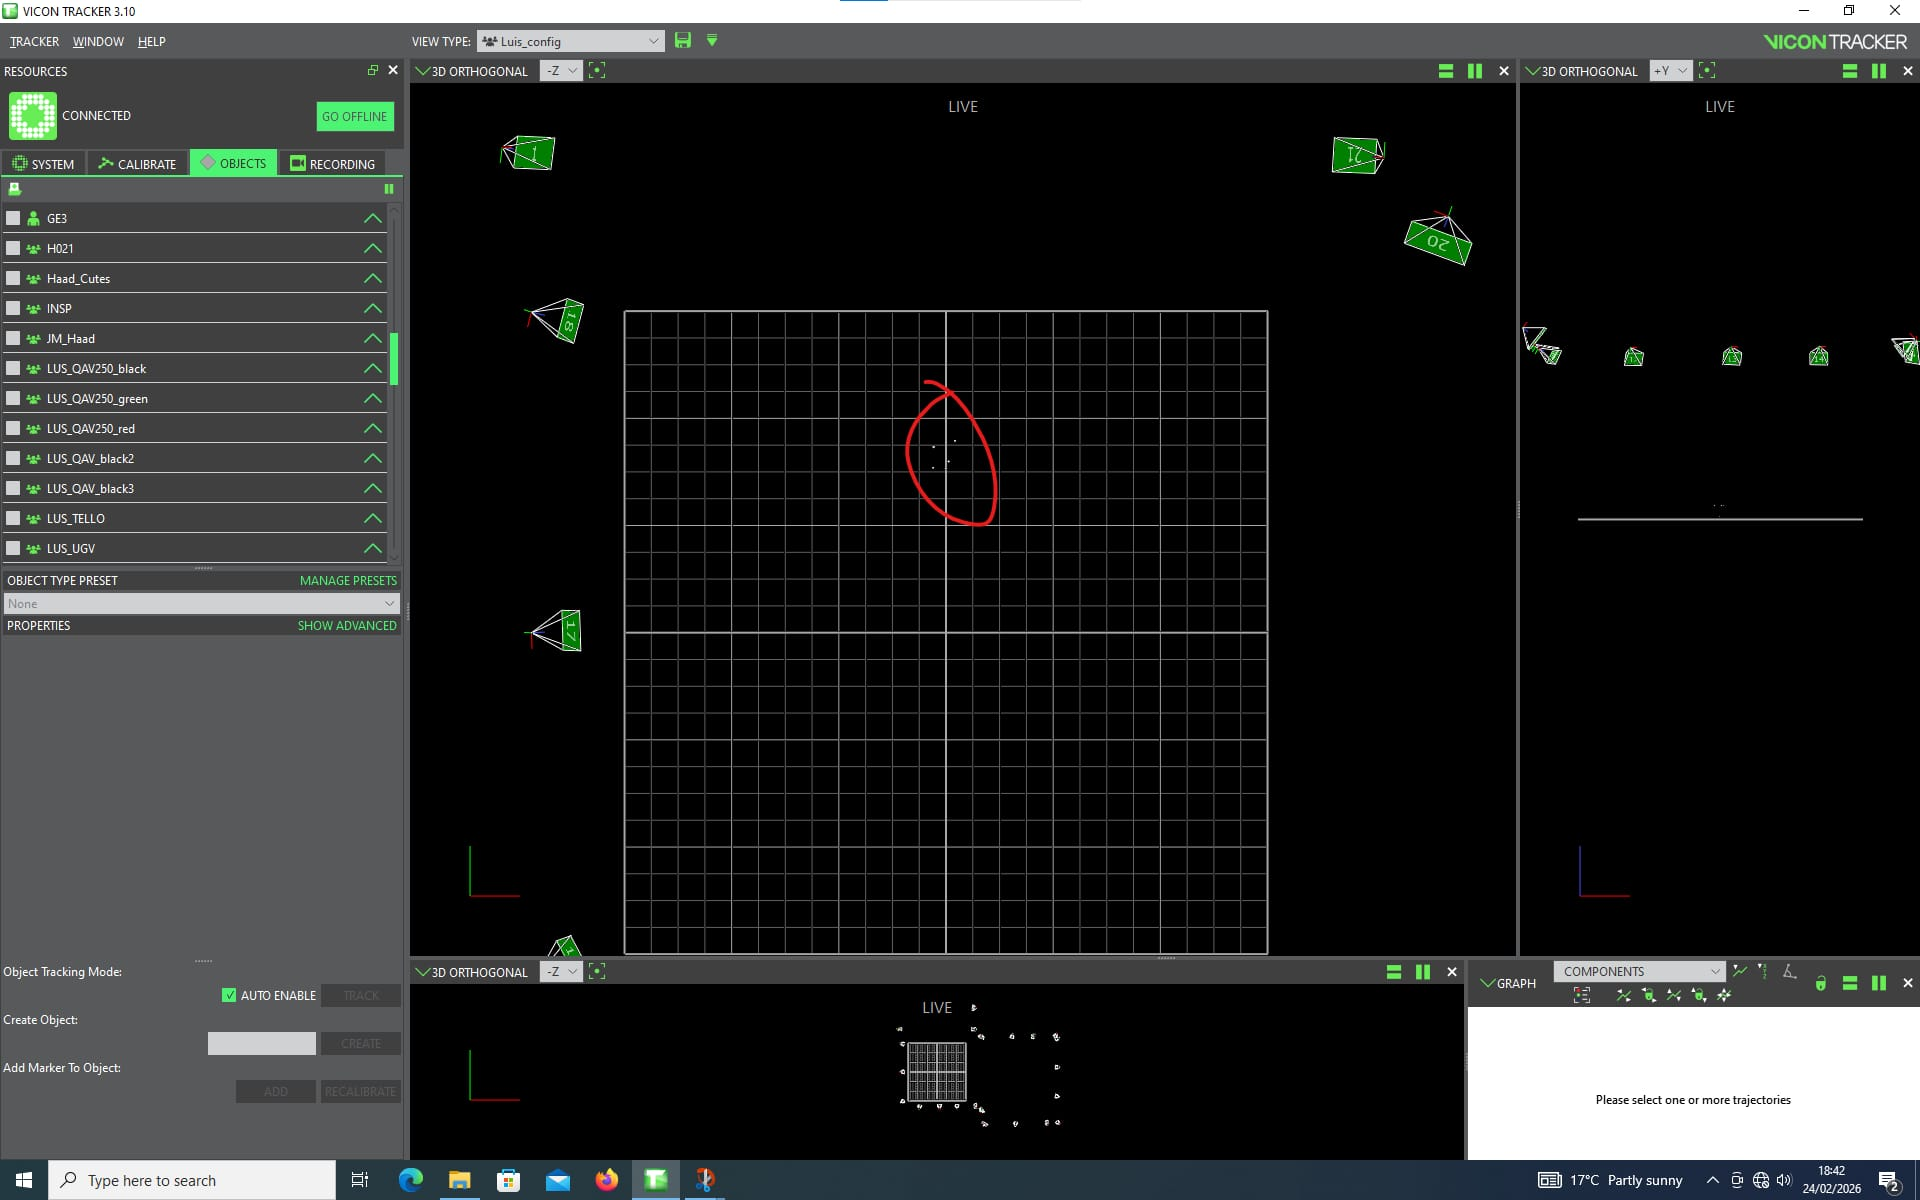
\includegraphics[width=1\linewidth]{Images/WhatsApp Image 2026-02-24 at 19.06.16.jpeg}
    \caption{Image of IR markers spotted in viewport.}
    \label{fig:21}
\end{figure}

Select the points by alt-clicking across them. It should show what cameras is currently tracking them, like in figure \ref{fig:22}.
\begin{figure}[H]
    \centering
    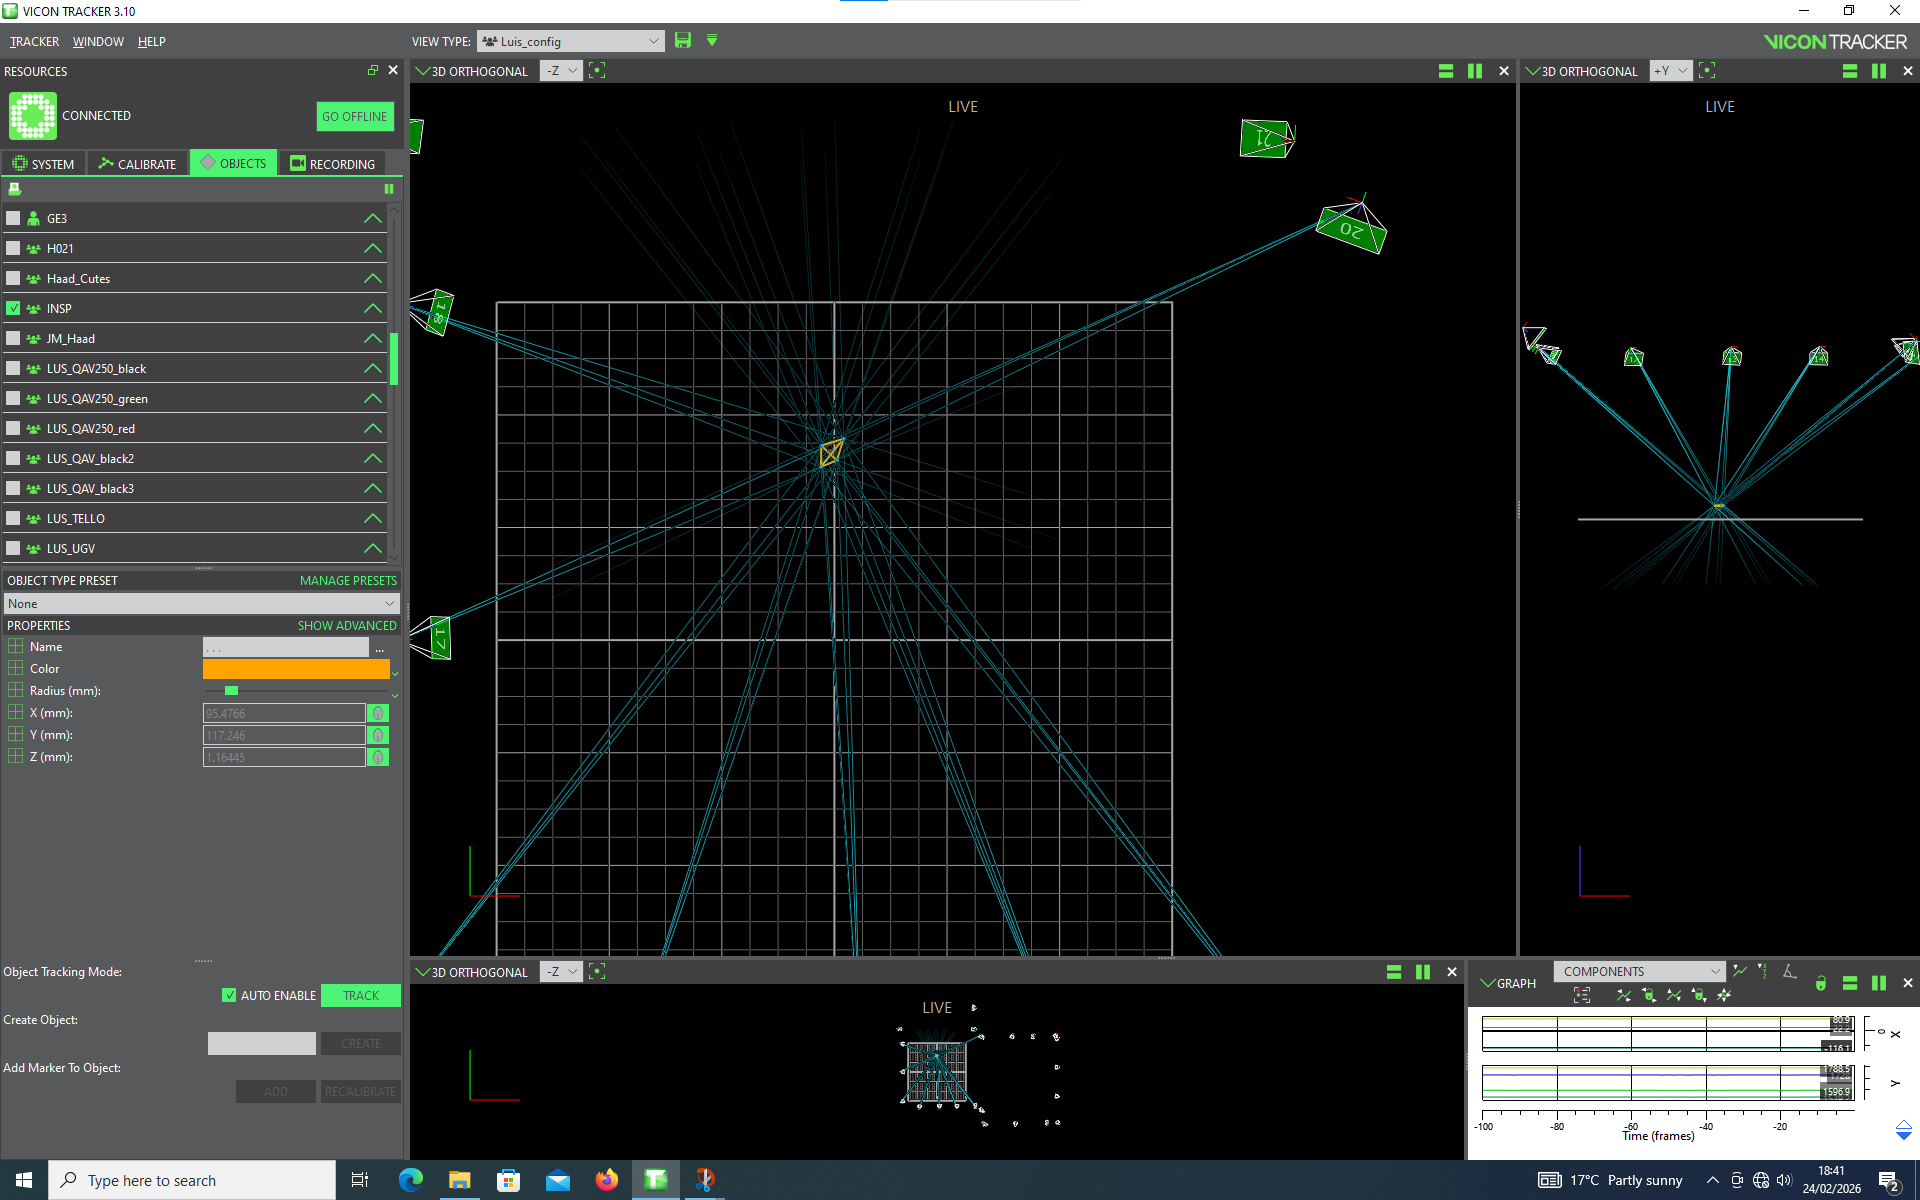
\includegraphics[width=1\linewidth]{Images/13 Alt click to track object.png}
    \caption{Image of IR Markers being selected.}
    \label{fig:22}
\end{figure}


Align your focus to the bottom left of the screen, seen in figure \ref{fig:24}. Type down the name of your object, and the \textit{CREATE} button should be enabled like in figure \ref{fig:25}. Press \textit{CREATE}, click \textit{SHARED}. 
\begin{figure}[H]
    \centering
    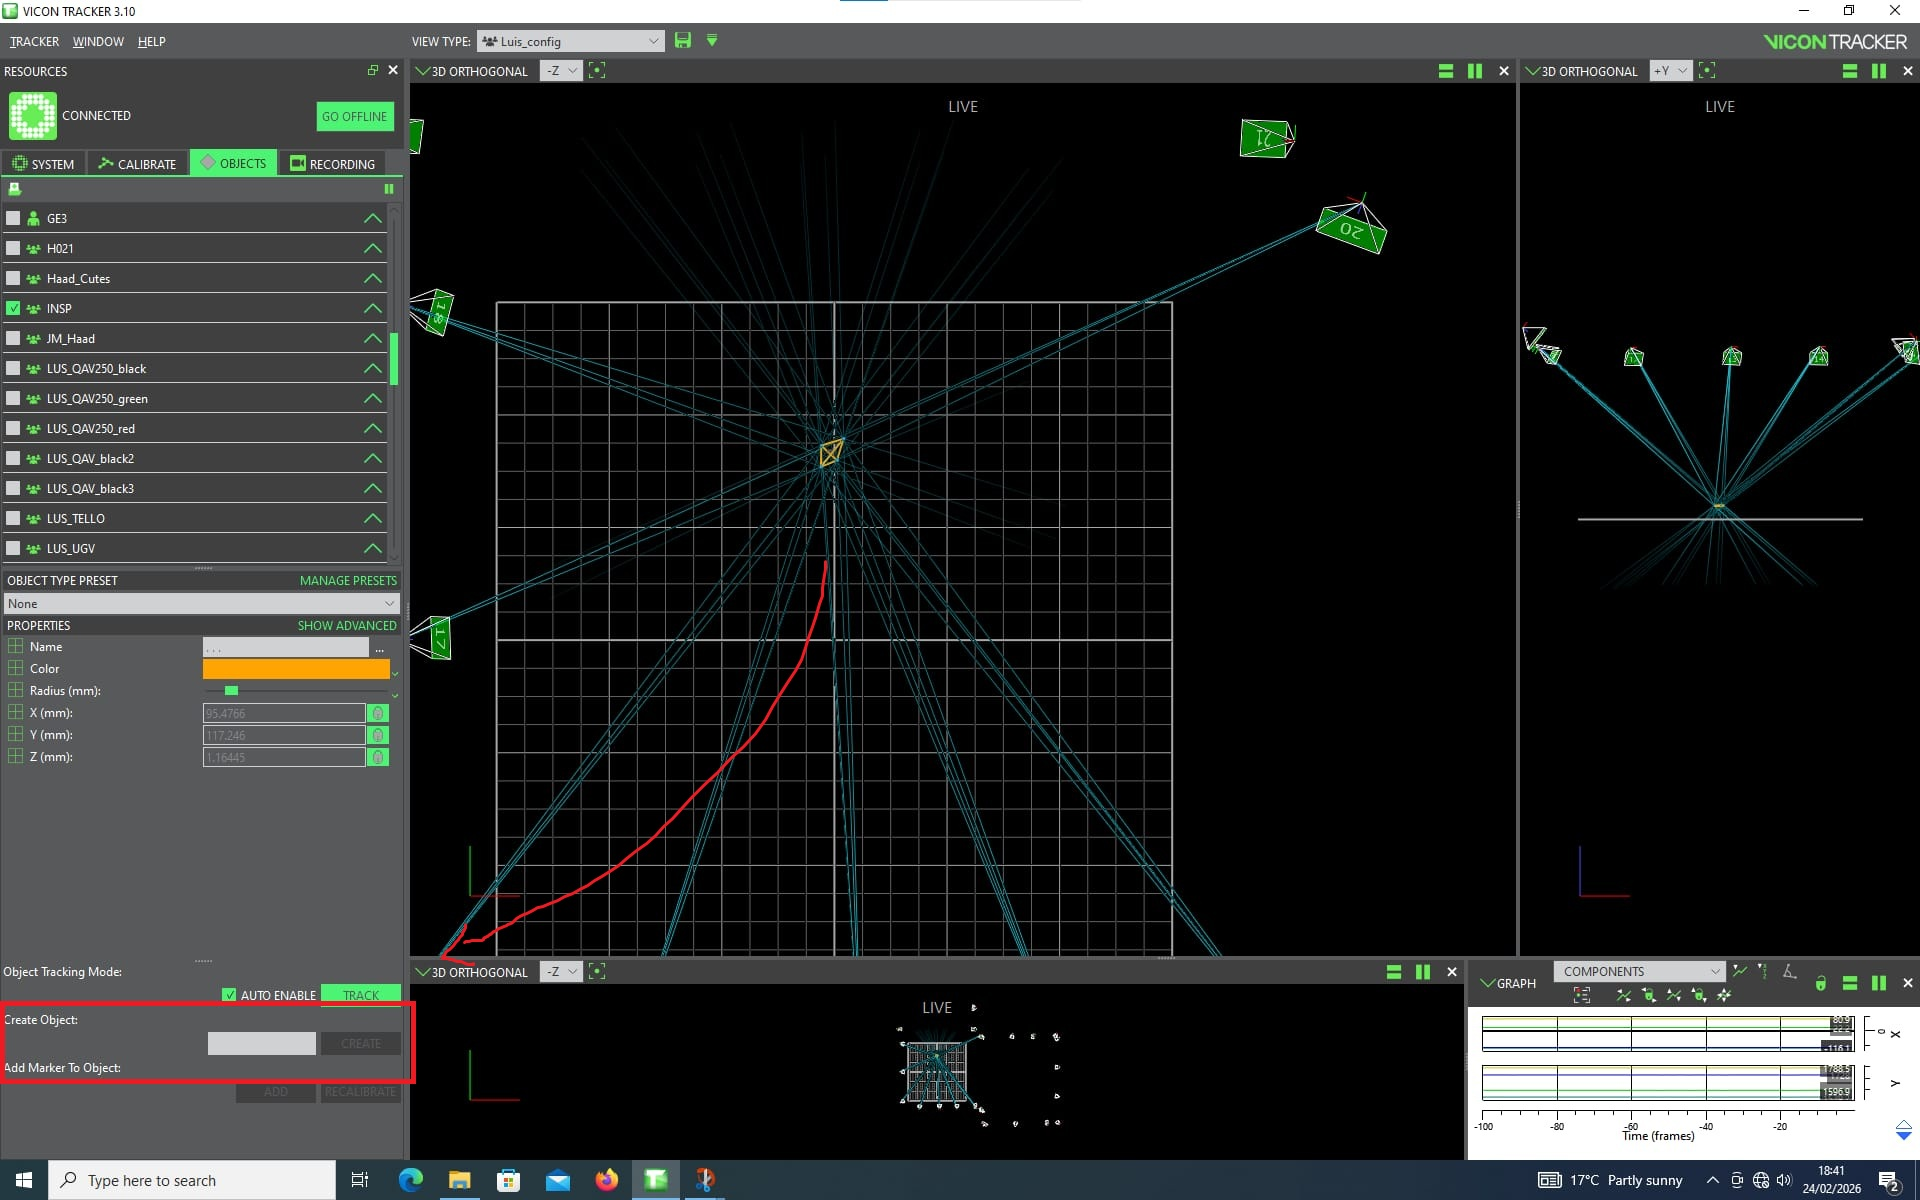
\includegraphics[width=1\linewidth]{Images/WhatsApp Image 2026-02-24 at 19.06.18 (2).jpeg}
    \caption{Image of the TRACK button}
    \label{fig:24}
\end{figure}
\begin{figure}[H]
    \centering
    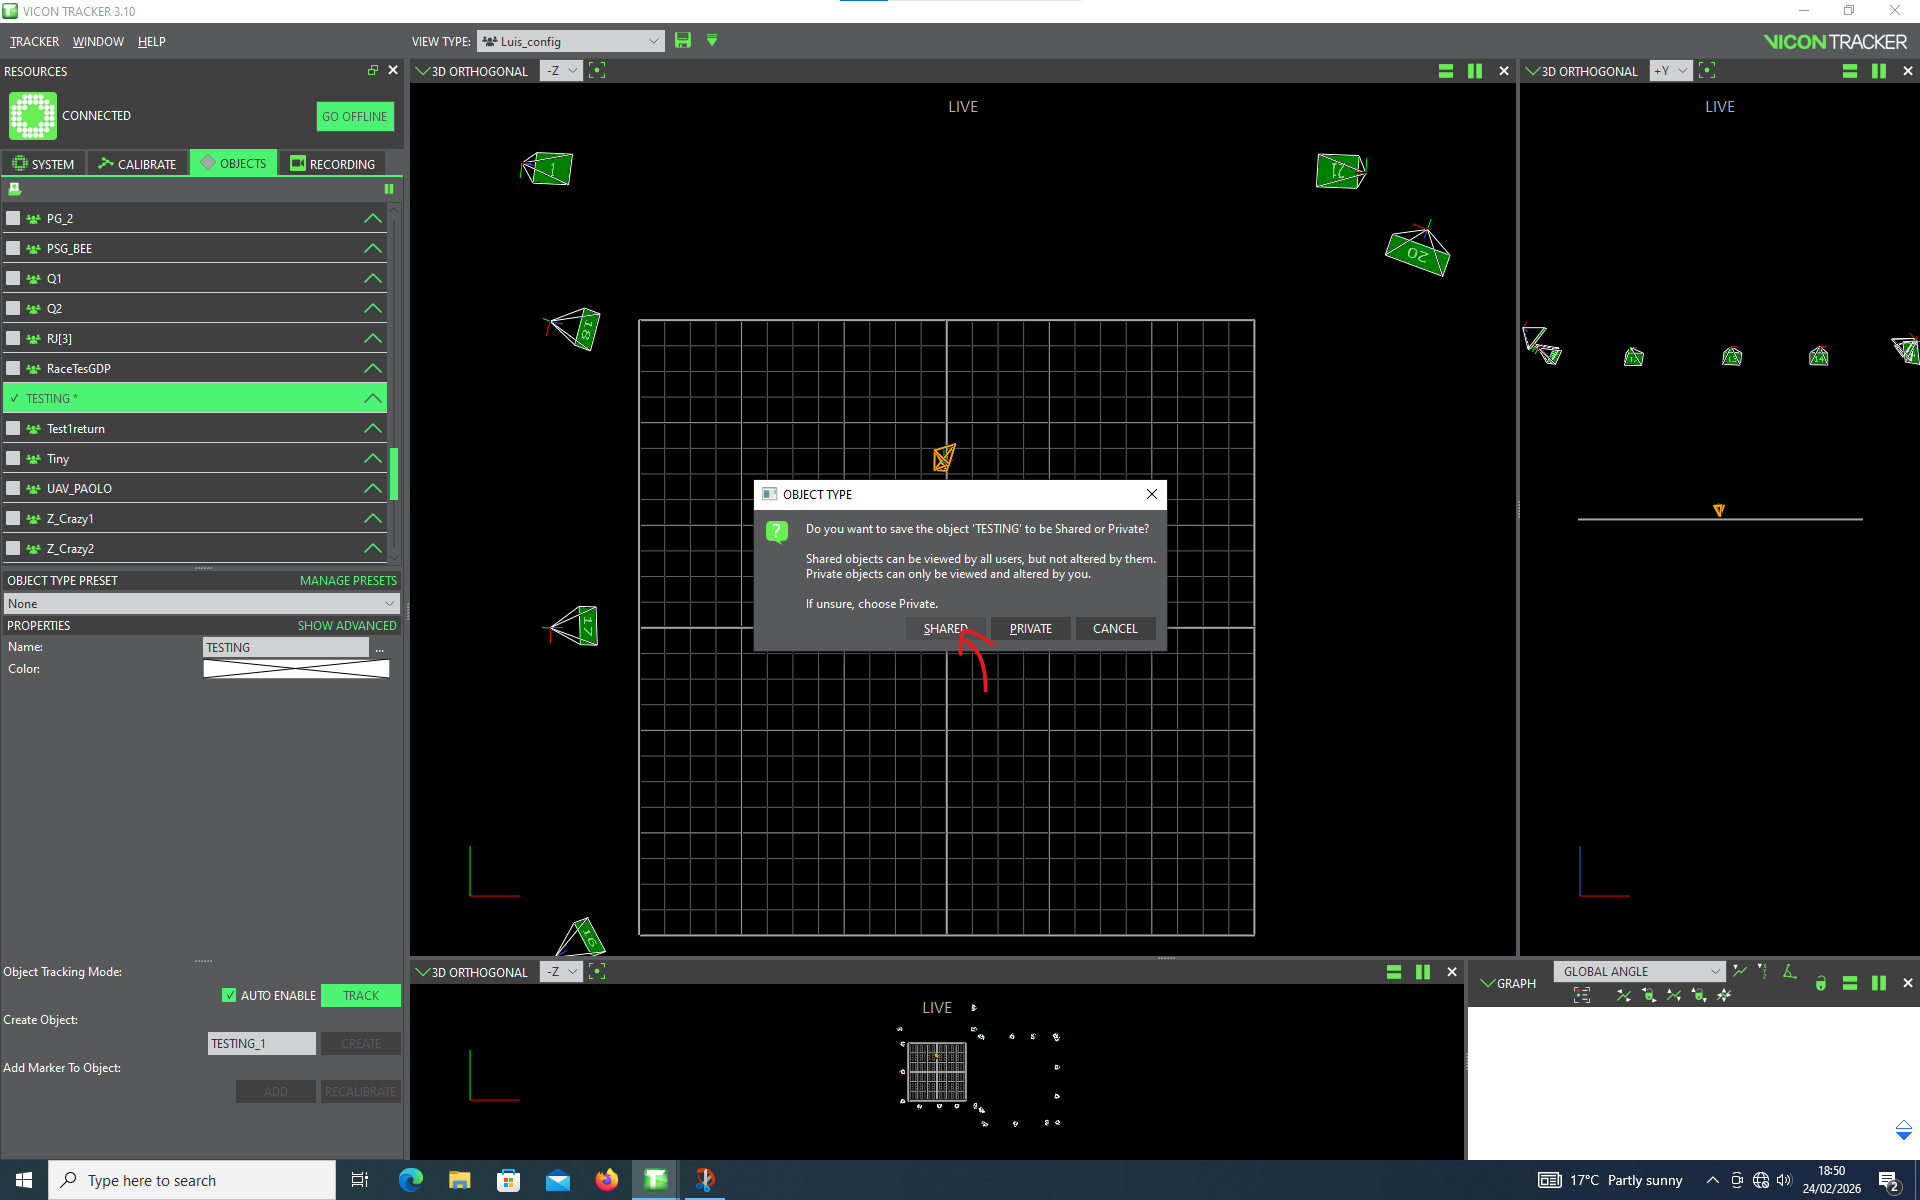
\includegraphics[width=1\linewidth]{Images/17 Shared saving.png}
    \caption{Image of creating object}
    \label{fig:25}
\end{figure}
From the list of objects, search for your newly defined object, and save to the list as shown in figure \ref{fig:26}.
\begin{figure}[H]   
    \centering
    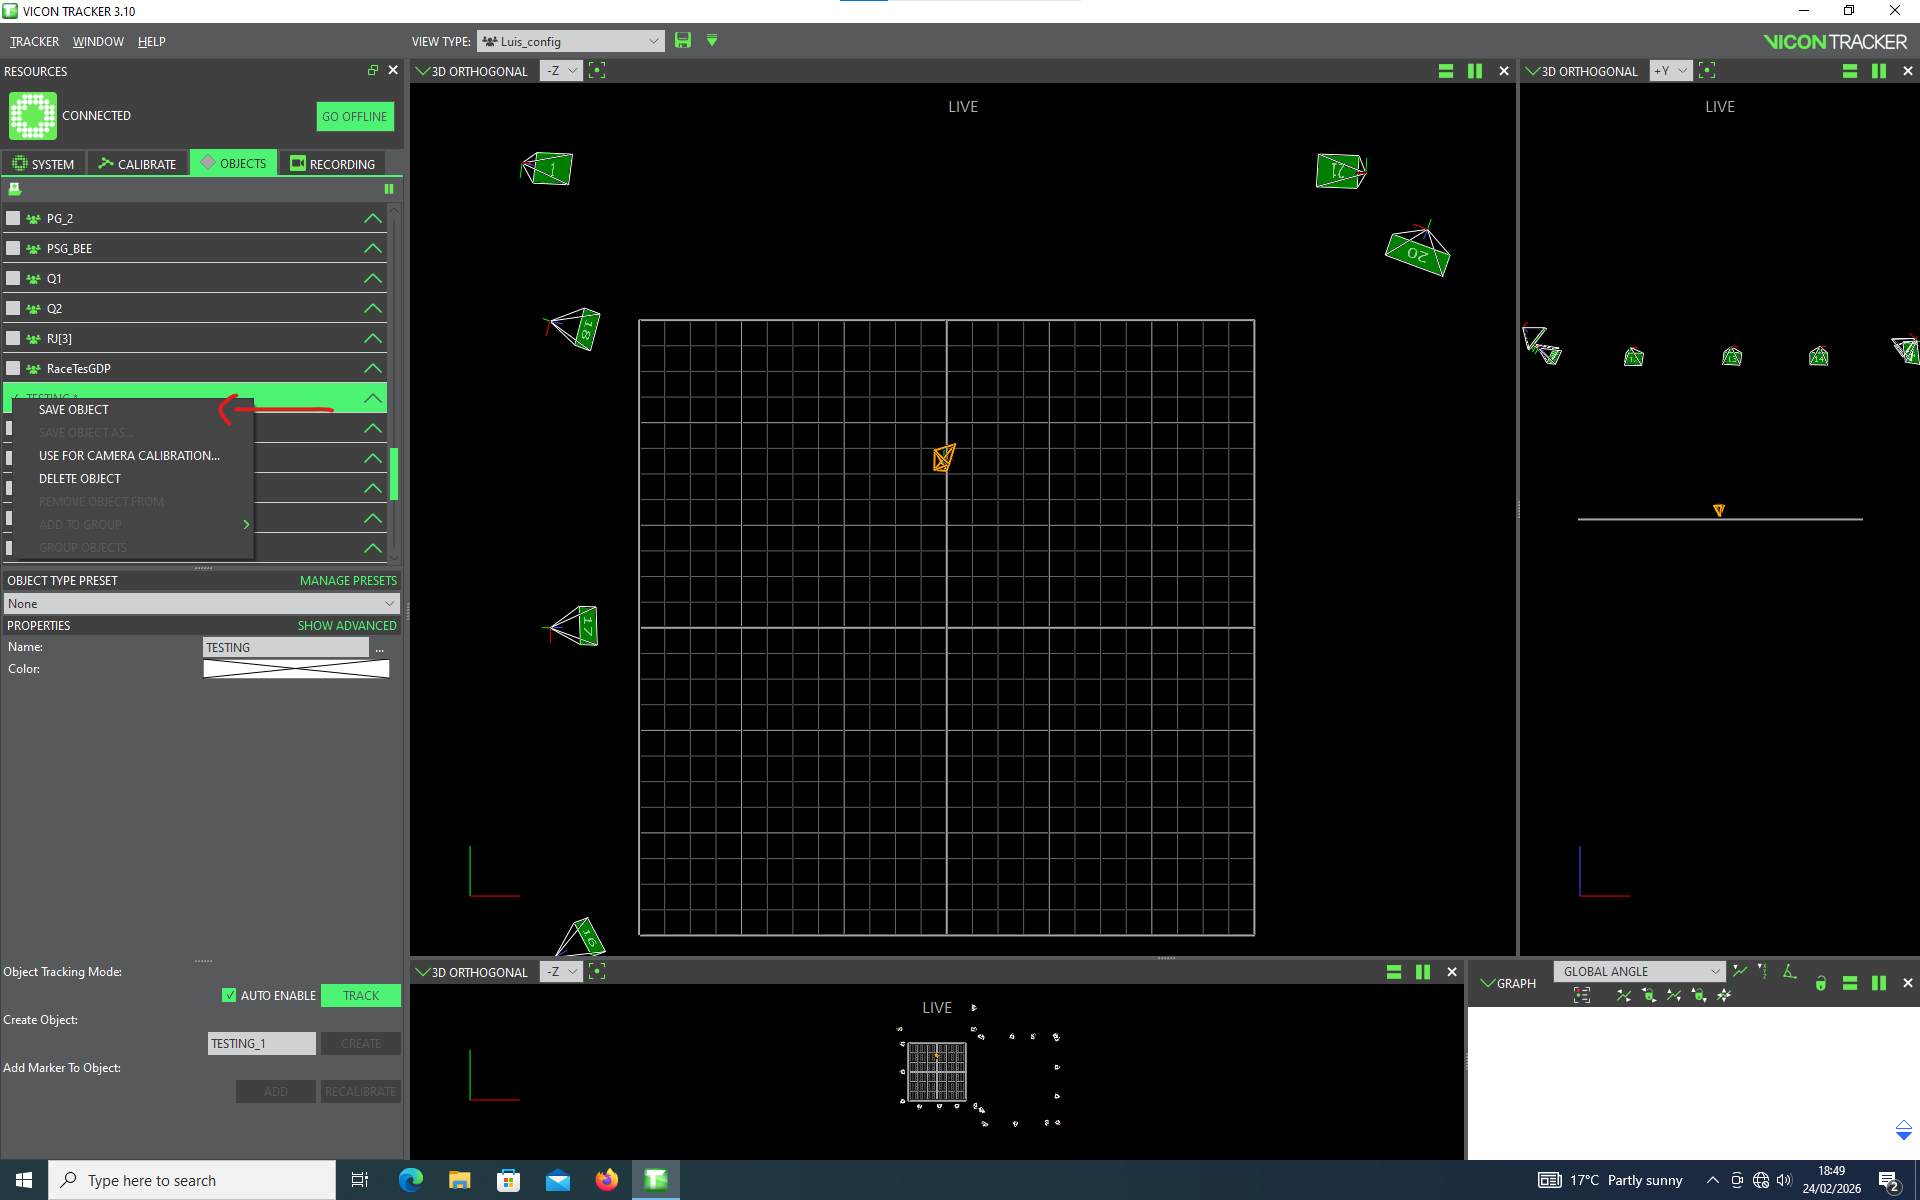
\includegraphics[width=1\linewidth]{Images/16 Save your object.png}
    \caption{Image of saving from object list.}
    \label{fig:26}
\end{figure}
 From this, your object is now integrated within the list of objects created by everyone else in the lab! I have been advised that it is good practice to have your object name to be around 4 letters, although I have seen names longer than 4. Luis will also thank you if you name your drones beginning with Z, so that it does not bring the ordering of the drones into a chaotic list. 
\subsection{Finishing}
Ensure you pack your Wand back into the box and return where you found it, sign out of the computer, remove all the obstacle and drones placed inside the flight arena, switch off the flight arena lights, turn off the Vicon Camera Power Switch. \\
\vspace{0.6cm}
From this point, the Vicon Server should be tracking your now defined object! This information can be broadcasted through Ethernet cables and to your Ground Control Station via \textit{MAVPROXY} \& \textit{MAVLINK}, this is most likely your next step. This will be reflected in next section \ref{sec:GCS}.
\clearpage